% Options for packages loaded elsewhere
\PassOptionsToPackage{unicode}{hyperref}
\PassOptionsToPackage{hyphens}{url}
%
\documentclass[
]{article}
\usepackage{amsmath,amssymb}
\usepackage{iftex}
\ifPDFTeX
  \usepackage[T1]{fontenc}
  \usepackage[utf8]{inputenc}
  \usepackage{textcomp} % provide euro and other symbols
\else % if luatex or xetex
  \usepackage{unicode-math} % this also loads fontspec
  \defaultfontfeatures{Scale=MatchLowercase}
  \defaultfontfeatures[\rmfamily]{Ligatures=TeX,Scale=1}
\fi
\usepackage{lmodern}
\ifPDFTeX\else
  % xetex/luatex font selection
\fi
% Use upquote if available, for straight quotes in verbatim environments
\IfFileExists{upquote.sty}{\usepackage{upquote}}{}
\IfFileExists{microtype.sty}{% use microtype if available
  \usepackage[]{microtype}
  \UseMicrotypeSet[protrusion]{basicmath} % disable protrusion for tt fonts
}{}
\makeatletter
\@ifundefined{KOMAClassName}{% if non-KOMA class
  \IfFileExists{parskip.sty}{%
    \usepackage{parskip}
  }{% else
    \setlength{\parindent}{0pt}
    \setlength{\parskip}{6pt plus 2pt minus 1pt}}
}{% if KOMA class
  \KOMAoptions{parskip=half}}
\makeatother
\usepackage{xcolor}
\usepackage[margin=1in]{geometry}
\usepackage{longtable,booktabs,array}
\usepackage{calc} % for calculating minipage widths
% Correct order of tables after \paragraph or \subparagraph
\usepackage{etoolbox}
\makeatletter
\patchcmd\longtable{\par}{\if@noskipsec\mbox{}\fi\par}{}{}
\makeatother
% Allow footnotes in longtable head/foot
\IfFileExists{footnotehyper.sty}{\usepackage{footnotehyper}}{\usepackage{footnote}}
\makesavenoteenv{longtable}
\usepackage{graphicx}
\makeatletter
\def\maxwidth{\ifdim\Gin@nat@width>\linewidth\linewidth\else\Gin@nat@width\fi}
\def\maxheight{\ifdim\Gin@nat@height>\textheight\textheight\else\Gin@nat@height\fi}
\makeatother
% Scale images if necessary, so that they will not overflow the page
% margins by default, and it is still possible to overwrite the defaults
% using explicit options in \includegraphics[width, height, ...]{}
\setkeys{Gin}{width=\maxwidth,height=\maxheight,keepaspectratio}
% Set default figure placement to htbp
\makeatletter
\def\fps@figure{htbp}
\makeatother
\setlength{\emergencystretch}{3em} % prevent overfull lines
\providecommand{\tightlist}{%
  \setlength{\itemsep}{0pt}\setlength{\parskip}{0pt}}
\setcounter{secnumdepth}{5}
\usepackage{booktabs}
\usepackage{longtable}
\usepackage{array}
\usepackage{multirow}
\usepackage{wrapfig}
\usepackage{float}
\usepackage{colortbl}
\usepackage{pdflscape}
\usepackage{tabu}
\usepackage{threeparttable}
\usepackage{threeparttablex}
\usepackage[normalem]{ulem}
\usepackage{makecell}
\usepackage{xcolor}
\ifLuaTeX
  \usepackage{selnolig}  % disable illegal ligatures
\fi
\IfFileExists{bookmark.sty}{\usepackage{bookmark}}{\usepackage{hyperref}}
\IfFileExists{xurl.sty}{\usepackage{xurl}}{} % add URL line breaks if available
\urlstyle{same}
\hypersetup{
  pdftitle={Course Evaluation Results},
  pdfauthor={Allan Omondi},
  hidelinks,
  pdfcreator={LaTeX via pandoc}}

\title{Course Evaluation Results}
\author{Allan Omondi}
\date{2023-10-02}

\begin{document}
\maketitle

{
\setcounter{tocdepth}{2}
\tableofcontents
}
\begin{longtable}[]{@{}
  >{\raggedright\arraybackslash}p{(\columnwidth - 2\tabcolsep) * \real{0.5488}}
  >{\raggedright\arraybackslash}p{(\columnwidth - 2\tabcolsep) * \real{0.4512}}@{}}
\toprule\noalign{}
\begin{minipage}[b]{\linewidth}\raggedright
Key
\end{minipage} & \begin{minipage}[b]{\linewidth}\raggedright
Value
\end{minipage} \\
\midrule\noalign{}
\endhead
\bottomrule\noalign{}
\endlastfoot
\textbf{Course} & Business Intelligence II \\
\textbf{Course Code} & BBT4206 \\
\textbf{Class} & BBIT 4.2 \\
\textbf{Semester Duration} & 21\textsuperscript{st} August 2023 to
28\textsuperscript{th} November 2023 \\
\textbf{Date of Evaluation} &
\begin{minipage}[t]{\linewidth}\raggedright
25\textsuperscript{th} September 2023 to 29\textsuperscript{th}
September 2023\\
(Week 6/14)\strut
\end{minipage} \\
\textbf{Total number of students who submitted the course evaluation} &
94 \\
\textbf{Total number of students registered in the AMS at the time of
the course evaluation} & 115 \\
\textbf{Response rate} & 81.73\% \\
\textbf{e-Learning URL} &
\url{https://elearning.strathmore.edu/course/view.php?id=6599} \\
\textbf{Data collection tool URL (for access to the raw data)} &
\url{https://elearning.strathmore.edu/mod/questionnaire/view.php?id=221958} \\
\textbf{Lecturer} & Dr Allan Omondi \\
\end{longtable}

\newpage

\begin{center}\rule{0.5\linewidth}{0.5pt}\end{center}

\section{Course Evaluation Score}\label{course-evaluation-score}

Overall Course Evaluation Score

Mean Score

Percentage

4.3839

87.6789

\begin{center}\rule{0.5\linewidth}{0.5pt}\end{center}

\subsection{Course Evaluation Scores per
Group}\label{course-evaluation-scores-per-group}

The \textbf{``Average Course Evaluation Rating''} variable in the plot
below indicates the score \textbf{per group} with a baseline of 4/5.

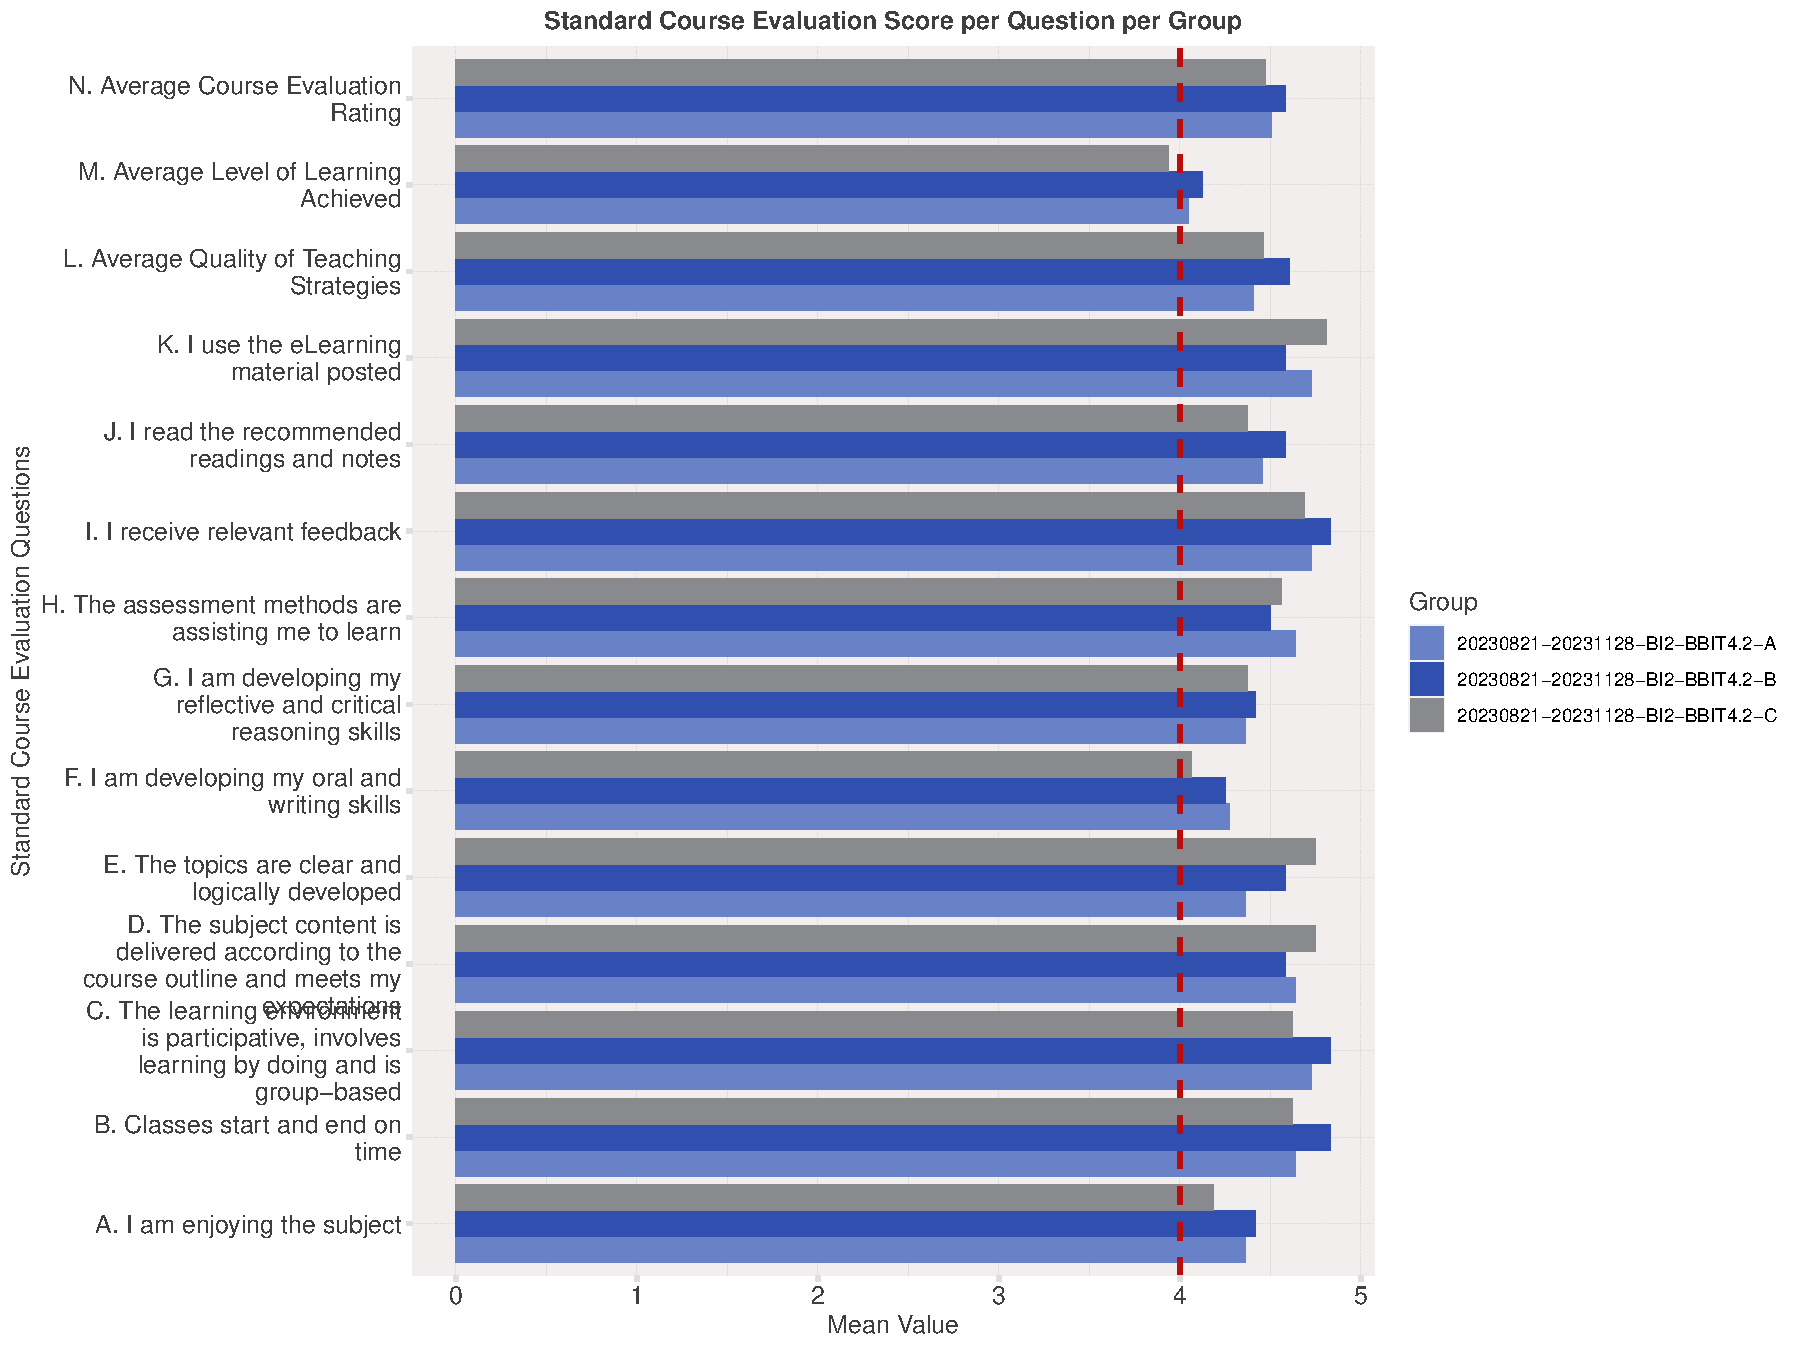
\includegraphics{AnalysisOfCourseEvaluation-Notebook_files/figure-latex/VisualizationsForCourseEvaluationResultsperClassGroup-1.pdf}

\newpage

The \textbf{``Average Course Evaluation Rating''} variable in the plot
below indicates the score \textbf{per gender} with a baseline of 4/5.

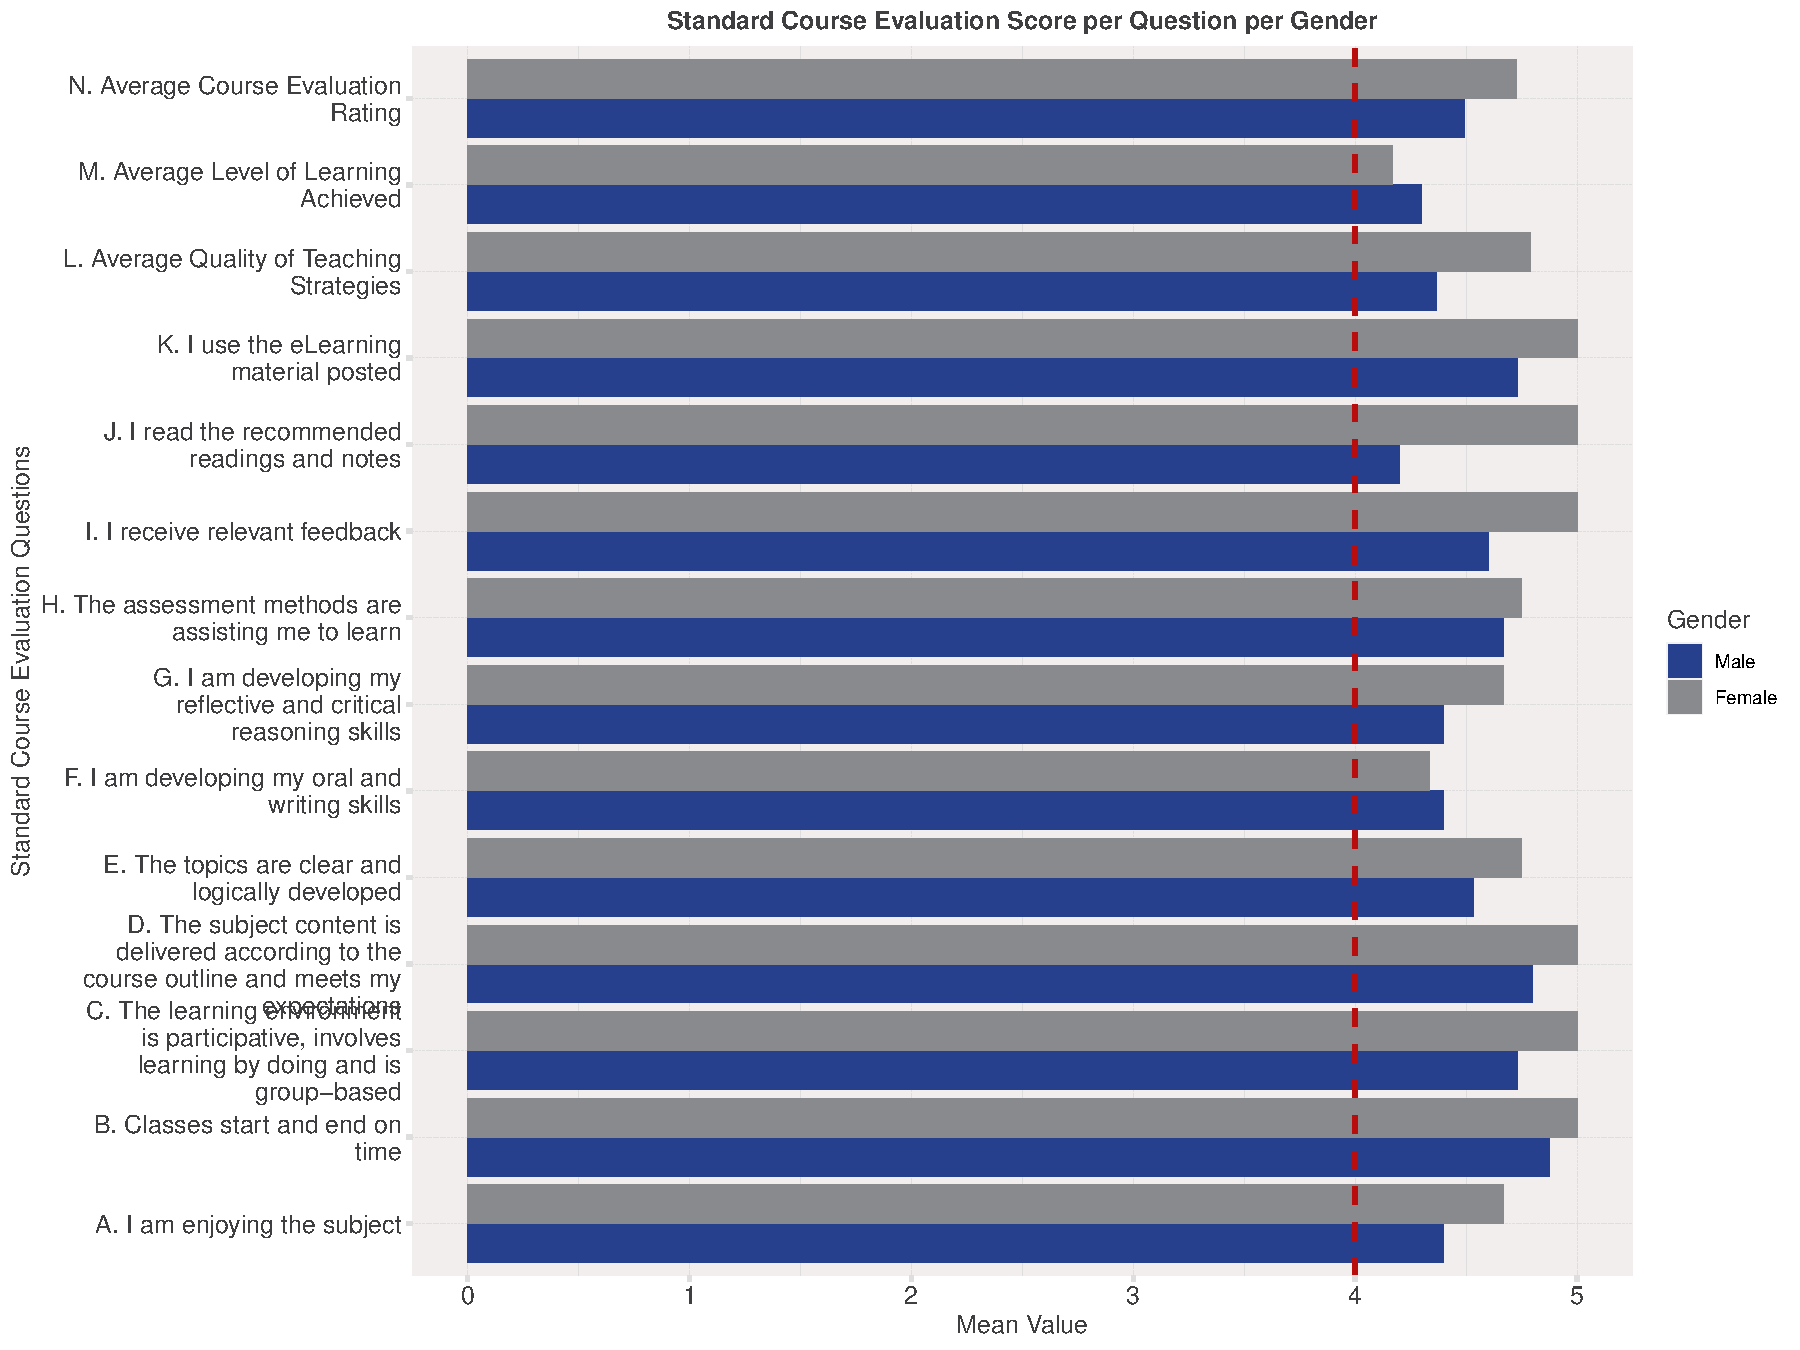
\includegraphics{AnalysisOfCourseEvaluation-Notebook_files/figure-latex/VisualizationsForCourseEvaluationResultsperGender-1.pdf}

\newpage

The plot below presents a drill-down of the class group into
\textbf{regular and exempt} students:

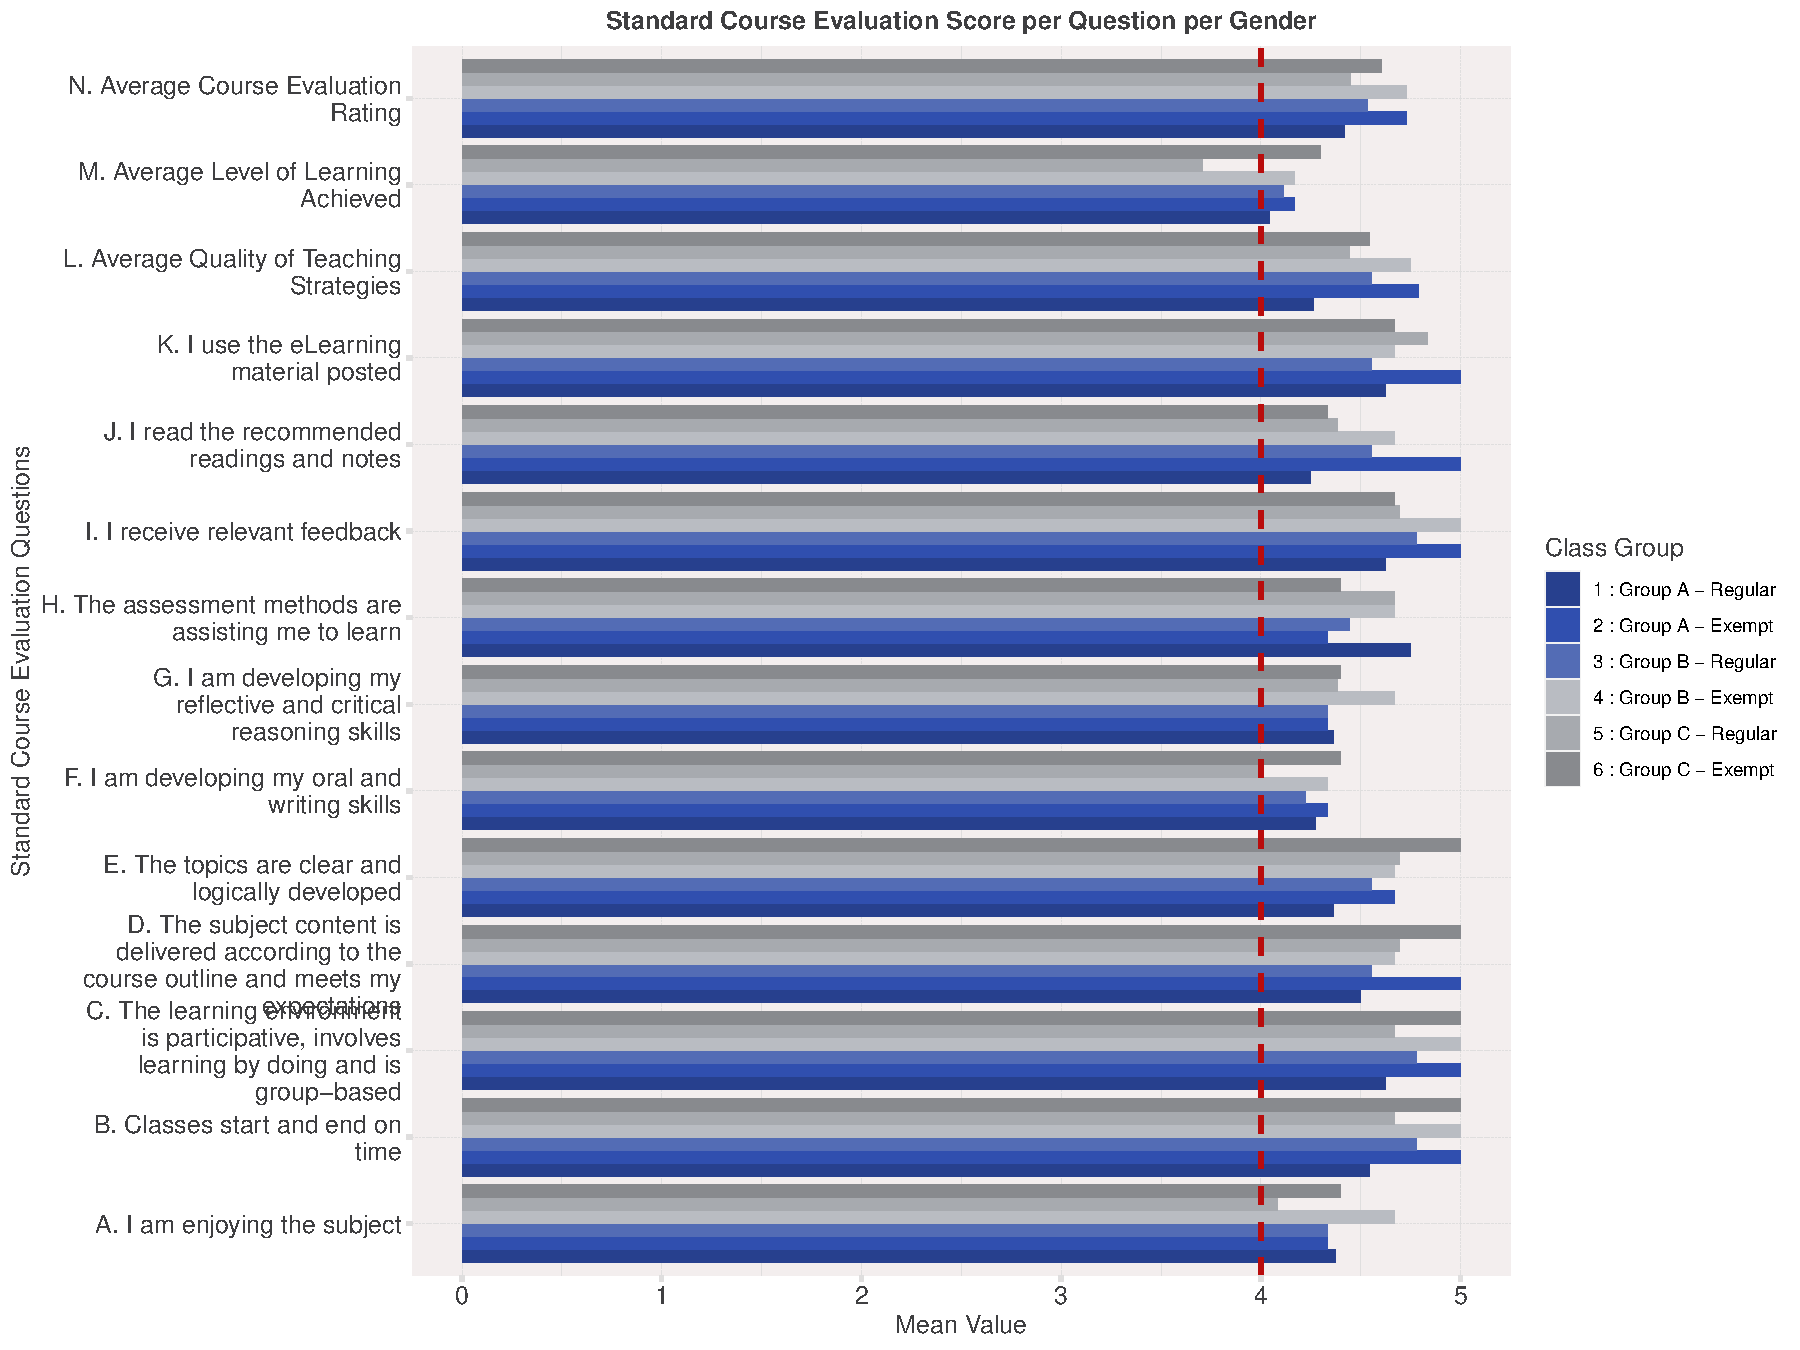
\includegraphics{AnalysisOfCourseEvaluation-Notebook_files/figure-latex/VisualizationsForCourseEvaluationResultsperGroup-1.pdf}

\newpage

\section{Correlations}\label{correlations}

The following variables have been renamed to fit the correlation plots:

\begin{itemize}
\item
  `A. Enjoying Subject` = `Q02\_General Questions-\textgreater A - 1. I
  am enjoying the subject`,
\item
  `B. Classes Start-End` = `Q02\_General Questions-\textgreater A - 2.
  Classes start and end on time`,
\item
  `C. Learning Environment` = `Q02\_General Questions-\textgreater A -
  3. The learning environment is participative, involves learning by
  doing and is group-based`,
\item
  `D. Content Delivery` = `Q02\_General Questions-\textgreater A - 4.
  The subject content is delivered according to the course outline and
  meets my expectations`,
\item
  `E. Clear Topics` = `Q02\_General Questions-\textgreater A - 5. The
  topics are clear and logically developed`,
\item
  `F. Oral and Writing` = `Q02\_General Questions-\textgreater A - 6. I
  am developing my oral and writing skills`,
\item
  `G. Critical Thinking` = `Q02\_General Questions-\textgreater A - 7. I
  am developing my reflective and critical reasoning skills`,
\item
  `H. Assessment Methods` = `Q02\_General Questions-\textgreater A - 8.
  The assessment methods are assisting me to learn`,
\item
  `I. Relevant Feedback` = `Q02\_General Questions-\textgreater A - 9. I
  receive relevant feedback`,
\item
  `J. Read Recommendations` = `Q02\_General Questions-\textgreater A -
  10. I read the recommended readings and notes`,
\item
  `L. eLearning Material` = `Q02\_General Questions-\textgreater A - 11.
  I use the eLearning material posted`,
\item
  `Understood Concept 1` = `Q03\_Level of Learning
  Achieved-\textgreater B - 1. Concept 1 of 4 - Ensemble Methods for
  Predictive Analytics`,
\item
  `Understood Concept 2` = `Q03\_Level of Learning
  Achieved-\textgreater B - 2. Concept 2 of 4 - Predictive Modelling
  Using R`,
\item
  `Teaching - Labs` = `Q04\_Quality of Teaching
  Strategies-\textgreater C - 1. Labs with comments that describe each
  step to be followed`,
\item
  `Labs with Submission` = `Q04\_Quality of Teaching
  Strategies-\textgreater C - 2. Labs that require you to put in effort
  to make a submission related to the content of the lab`,
\item
  `Git in Teams` =`Q04\_Quality of Teaching Strategies-\textgreater C -
  3. Labs that require you to use Git to work in a team`,
\item
  `Solo Labs` = `Q04\_Quality of Teaching Strategies-\textgreater C - 4.
  Labs that require you to work alone`,
\item
  `Quality of Lectures` = `Q04\_Quality of Teaching
  Strategies-\textgreater C - 5. The quality of the lectures given
  (quality measured by the breadth (the full span of knowledge of a
  subject) and depth (the extent to which specific topics are focused
  upon, amplified, and explored) of learning - NOT quality measured by
  how fun/comical/lively the lectures are)`,
\item
  `Recordings of Classes` = `Q04\_Quality of Teaching
  Strategies-\textgreater C - 6. The recordings of online classes`,
\item
  `Online Classes` = `Q04\_Quality of Teaching Strategies-\textgreater C
  - 7. Online classes in general`,
\item
  `Physical Classes` = `Q04\_Quality of Teaching
  Strategies-\textgreater C - 8. Face-to-Face classes in general`
\end{itemize}

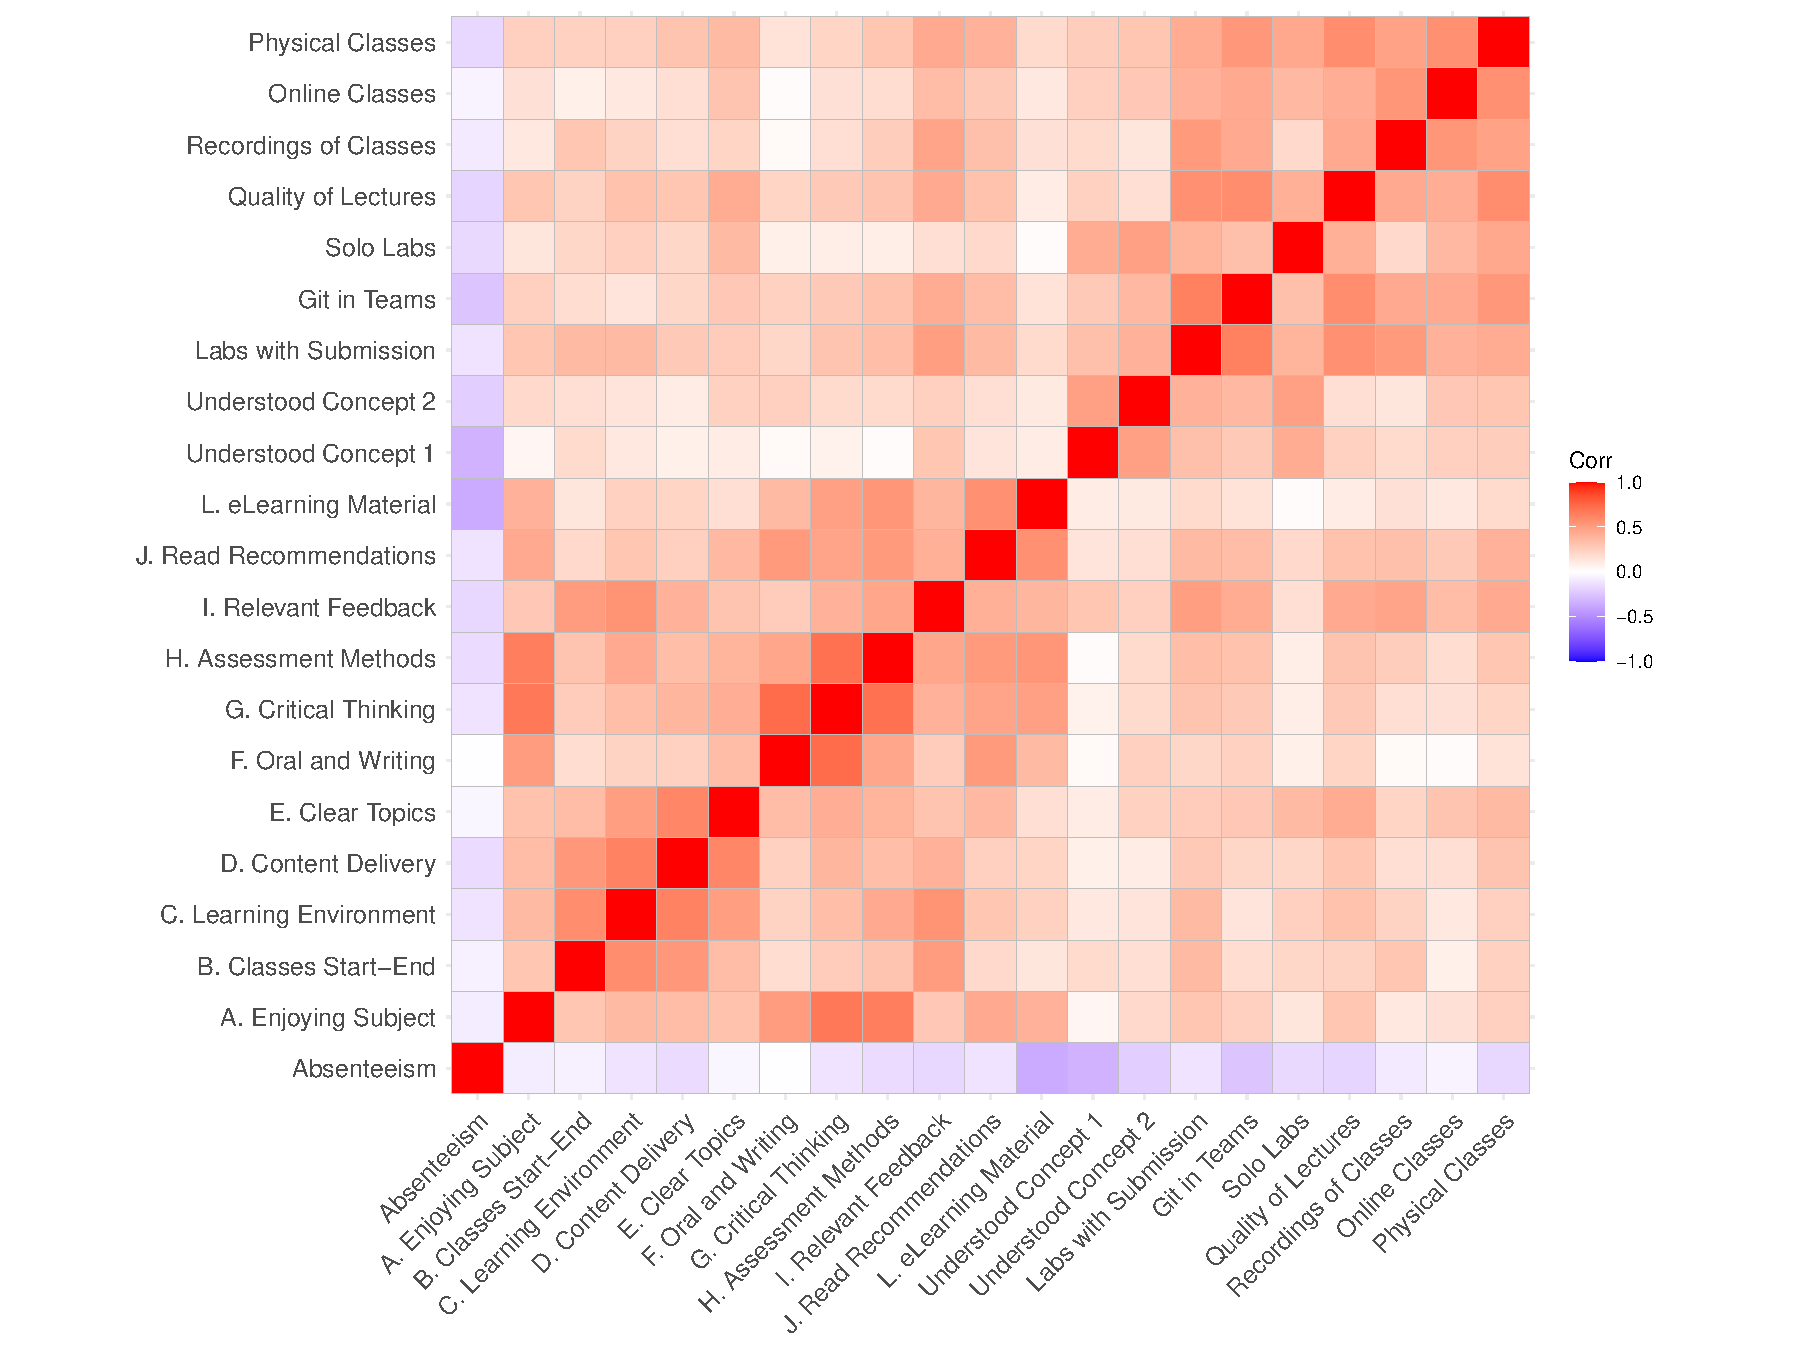
\includegraphics{AnalysisOfCourseEvaluation-Notebook_files/figure-latex/CorrelationMatrixWithoutFigures-1.pdf}

\newpage

The specifc correlation values are presented below:

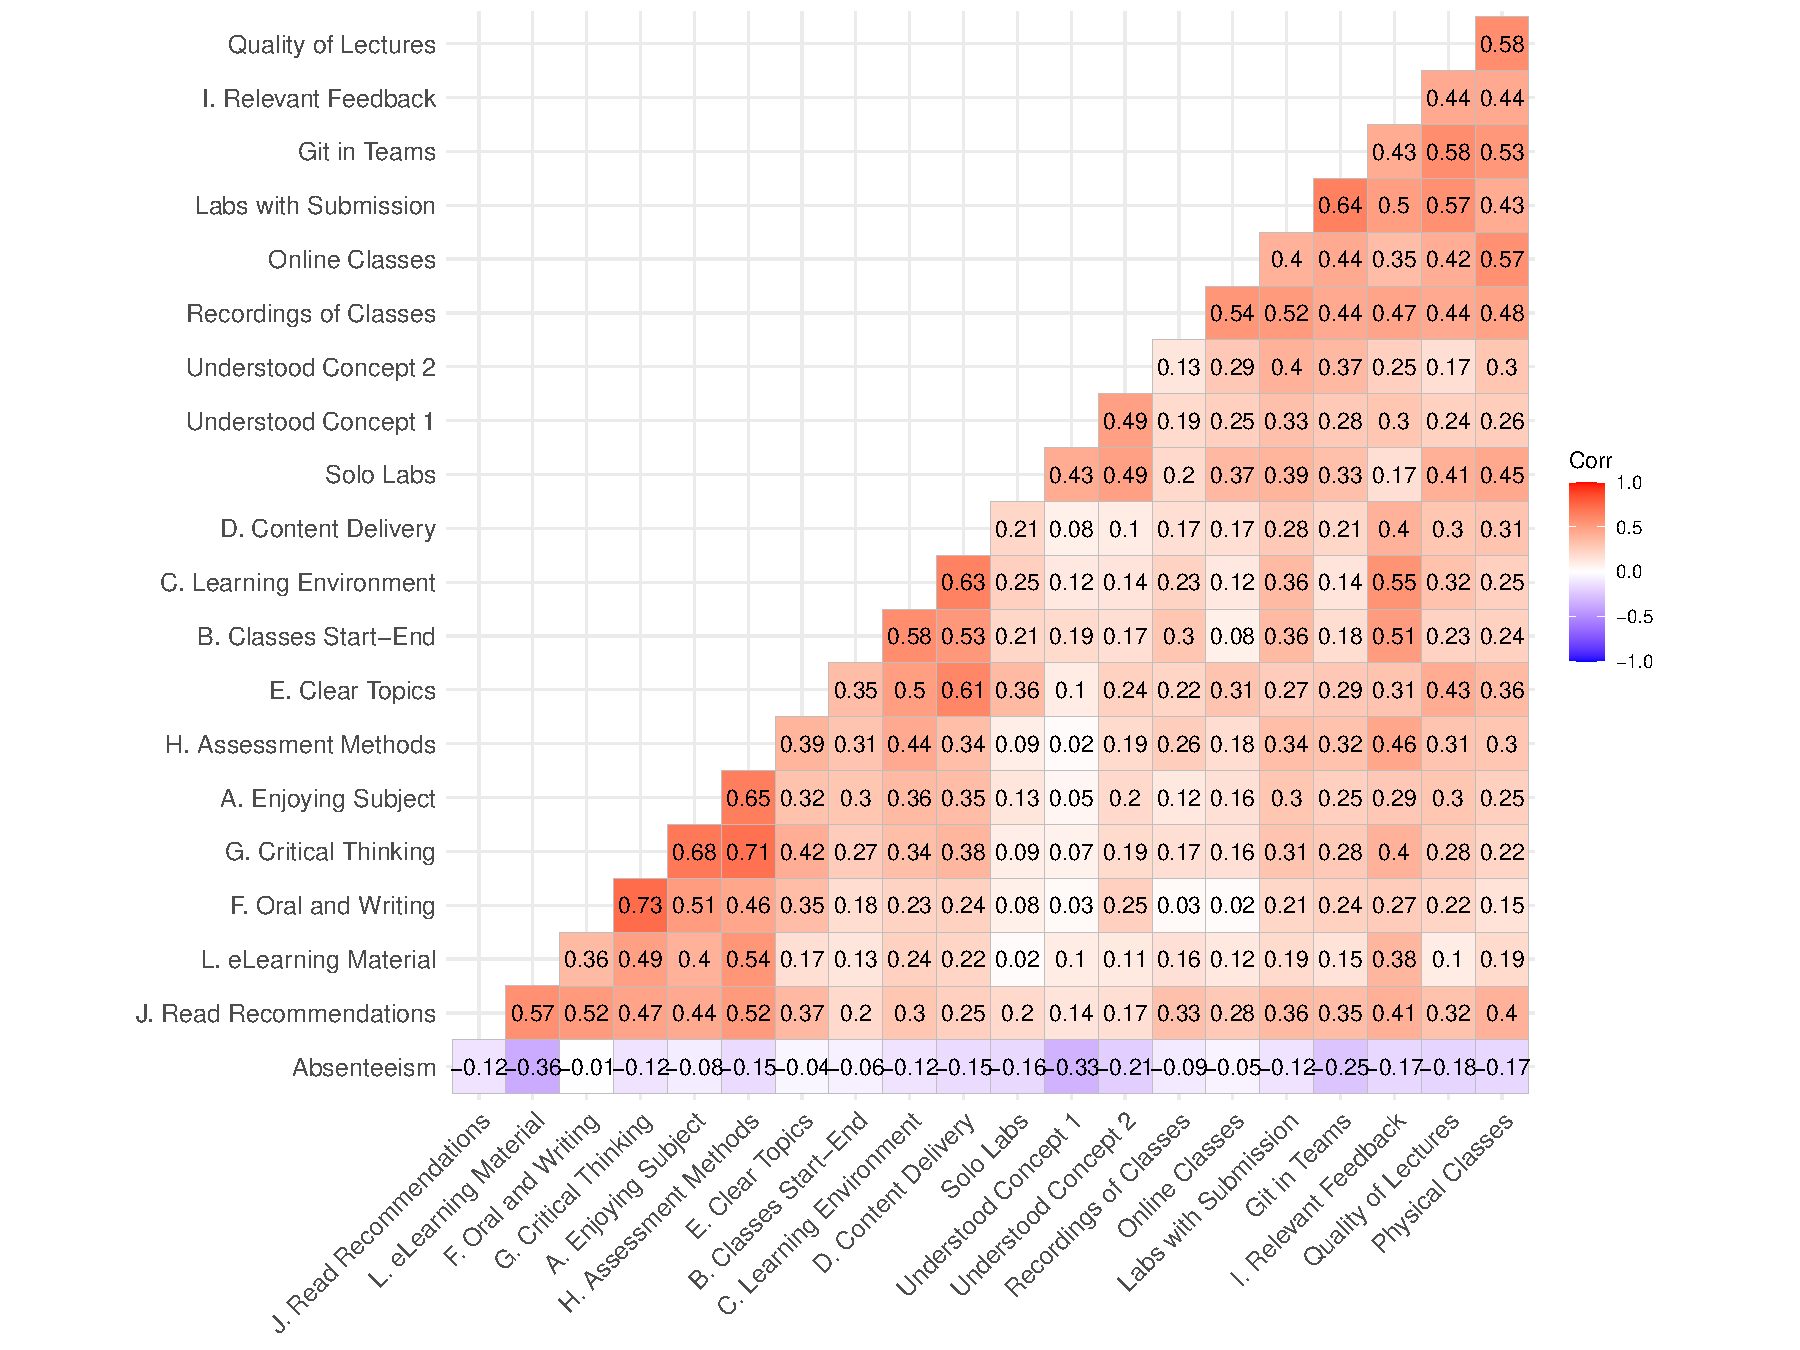
\includegraphics{AnalysisOfCourseEvaluation-Notebook_files/figure-latex/CorrelationMatrixWithFigures-1.pdf}

\subsection{Interesting Correlations}\label{interesting-correlations}

The following are hypothetical statements given that ``correlation does
not imply causation''.

\begin{itemize}
\item
  \textbf{.73 correlation} between ``I am developing my oral and writing
  skills'' and ``I am developing my reflective and critical reasoning
  skills'': \emph{Consider writing as formalized thinking.}
\item
  \textbf{.71 correlation} between ``The assessment methods are
  assisting me to learn'' and ``I am developing my reflective and
  critical reasoning skills'': \emph{The more effort students put into
  the assessment, the more they develop their reflective and critical
  reasoning skills.}
\item
  \textbf{.68 correlation} between ``I am enjoying the subject'' and ``I
  am developing my reflective and critical reasoning skills'': \emph{The
  more a student enjoys the subject, the more they consider their
  reflective and critical reasoning skills as developing.}
\item
  \textbf{.65 correlation} between ``The assessment methods are
  assisting me to learn'' and ``I am enjoying the subject'':
  \emph{Students who value the assessments enjoy the subject more.}
\item
  \textbf{.64 correlation} between ``Labs that require you to use Git to
  work in a team'' and ``Labs that require you to put in effort to make
  a submission related to the content of the lab'': \emph{The more
  students appreciate the use of Git for working in teams, the more they
  appreciate labs that require a submission to be made.}
\item
  \textbf{.61 correlation} between ``The subject content is delivered
  according to the course outline and meets my expectations'' and ``The
  topics are clear and logically developed'': \emph{The more the course
  outline is followed, the clearer and more logically developed the
  topics are.}
\item
  \textbf{-.33 correlation} between ``Concept 1 of 4 - Ensemble Methods
  for Predictive Analytics'' and ``Absenteeism'': \emph{Students who
  started the semester late (high absenteeism), had a harder time
  understanding concept 1 which was covered at the beginning of the
  semester.}
\item
  \textbf{-.36 correlation} between ``I use the e-learning material
  posted'' and ``absenteeism'': \emph{The higher the number of classes
  missed, the lower the student's engagement with content posted on
  e-learning}
\end{itemize}

Below are the two most extreme (positive and negative) correlations:

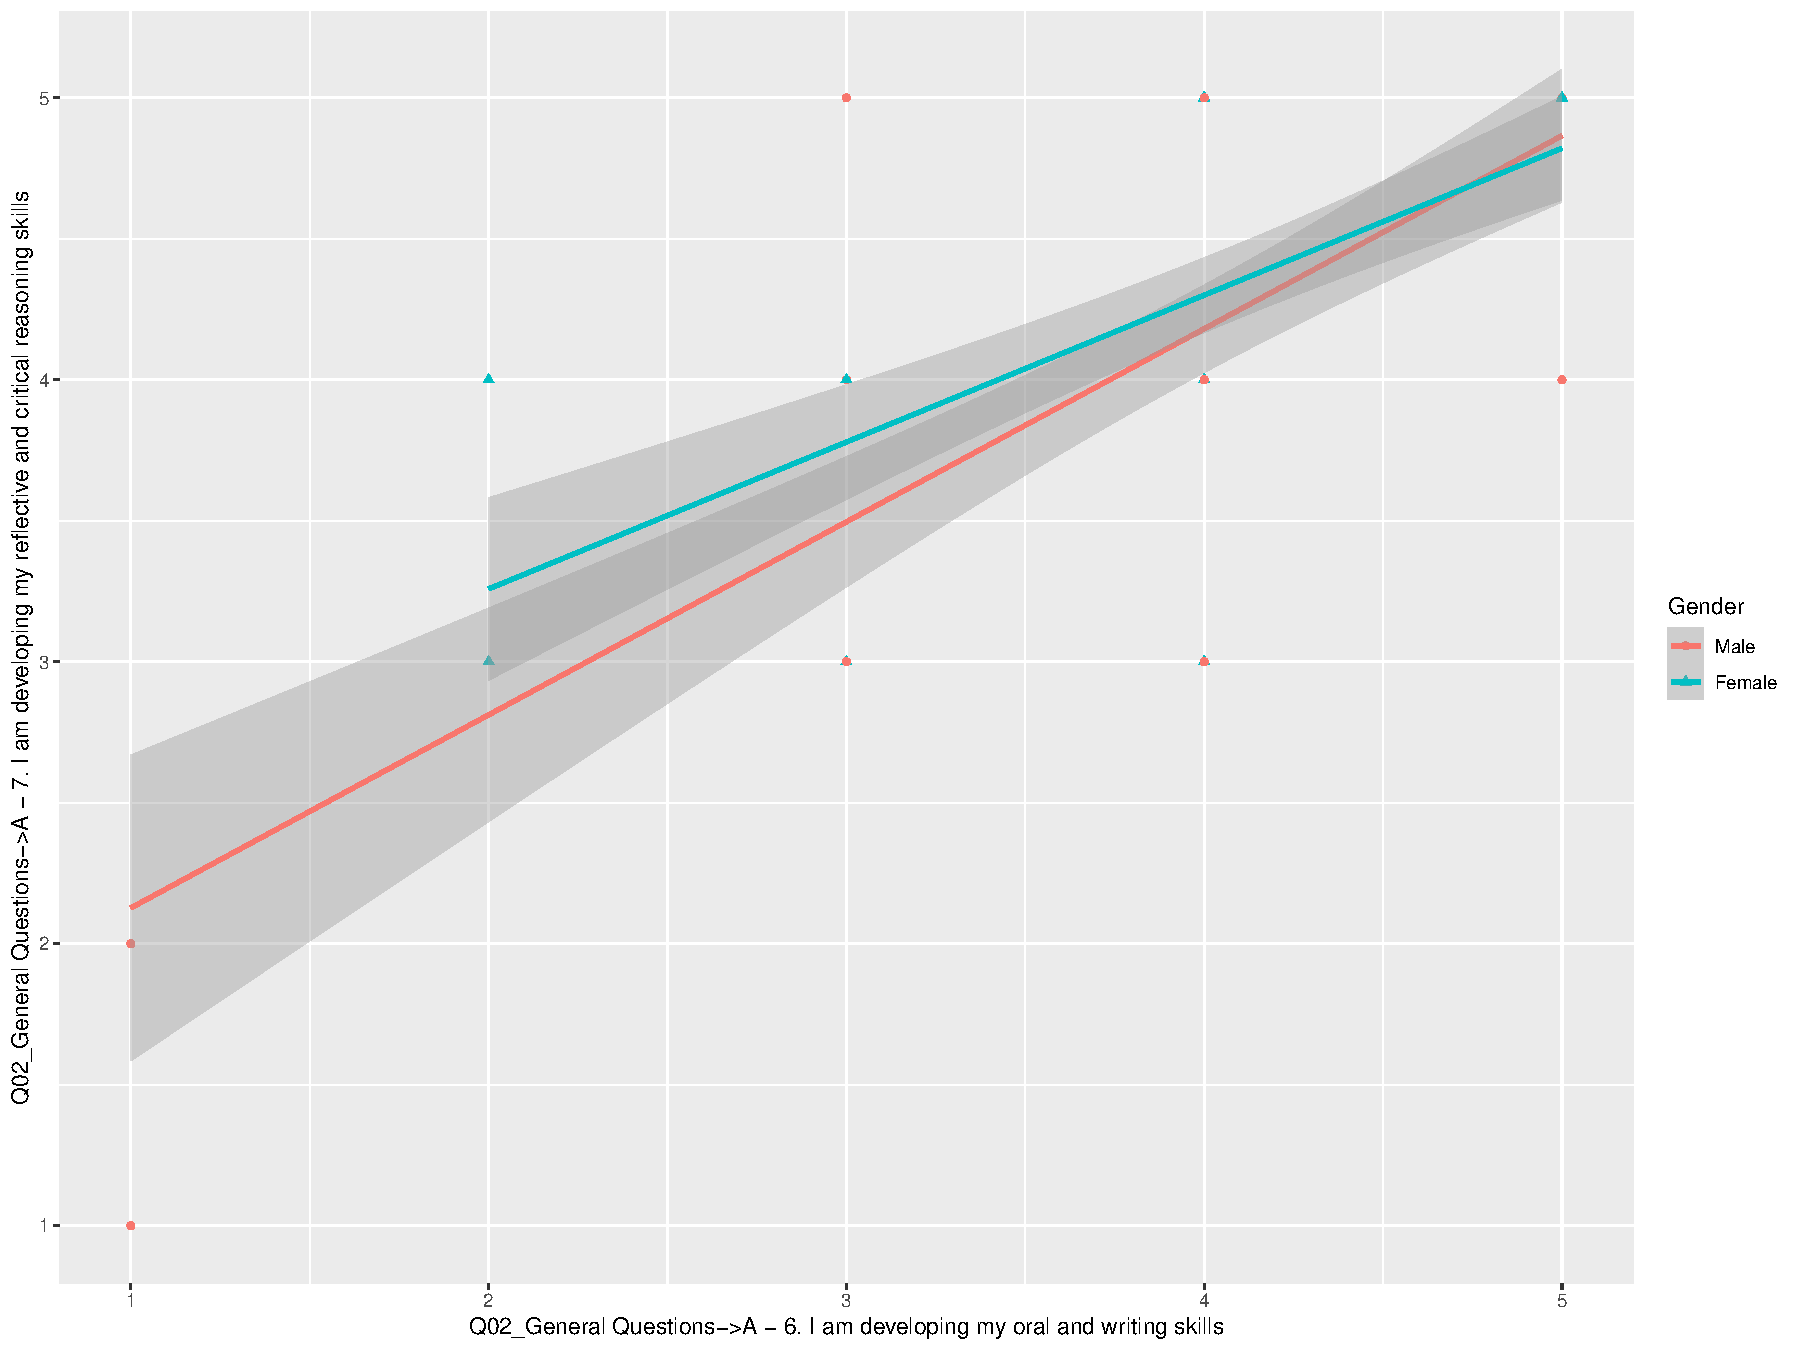
\includegraphics{AnalysisOfCourseEvaluation-Notebook_files/figure-latex/DrillDownCorr1-1.pdf}

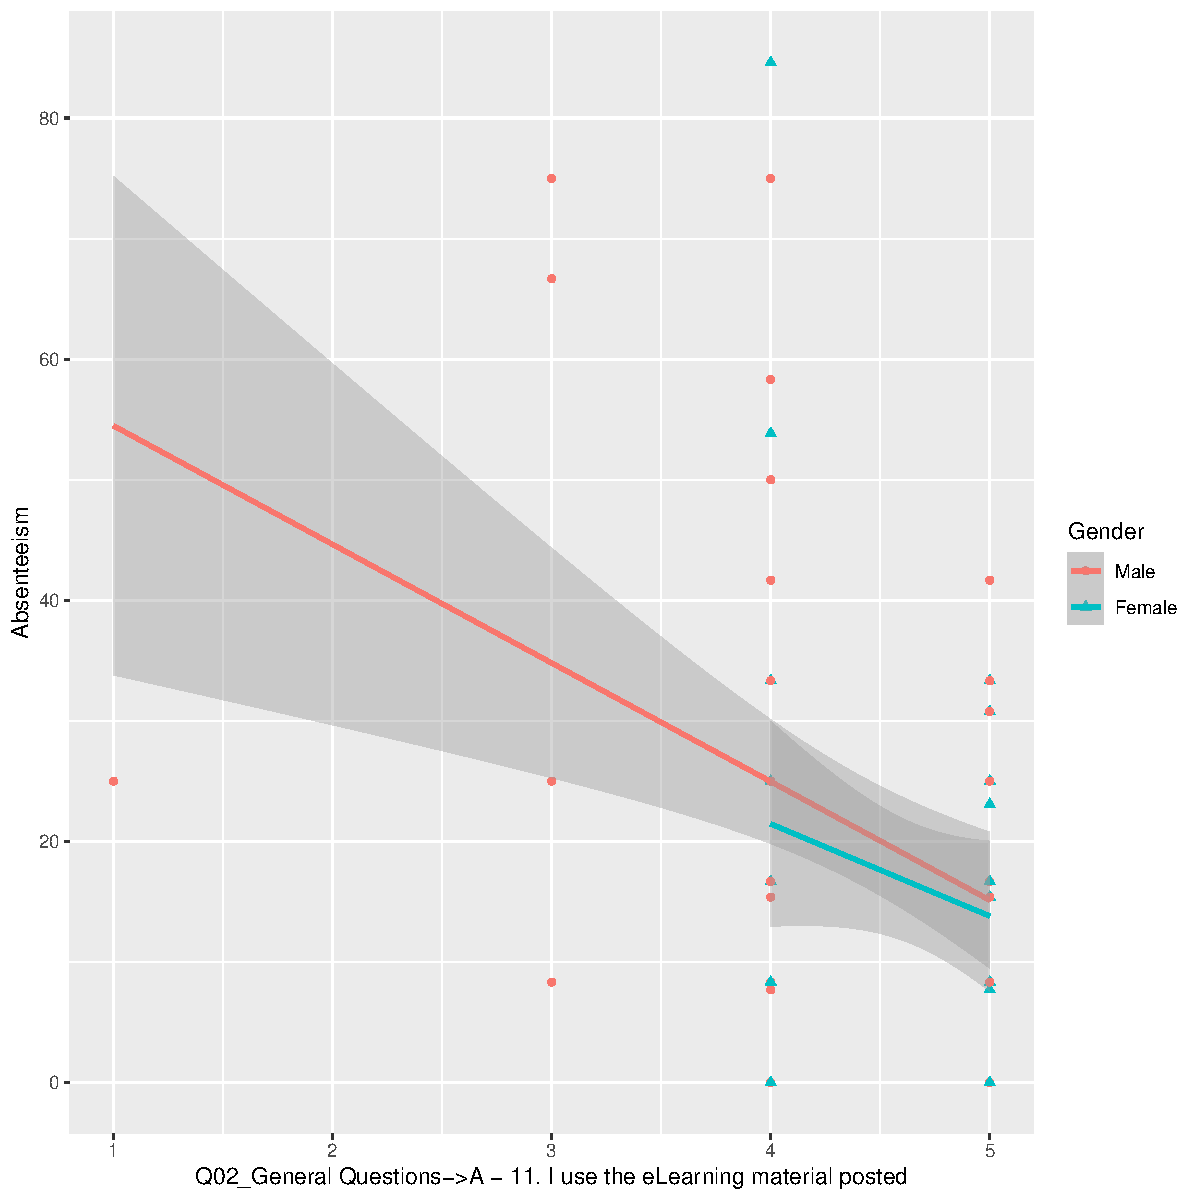
\includegraphics{AnalysisOfCourseEvaluation-Notebook_files/figure-latex/DrillDownCorr2-1.pdf}

\newpage

\subsection{Absenteeism Percentage}\label{absenteeism-percentage}

The lower the absenteeism, the more a student makes use of the
e-learning materials posted. And the more a student makes use of the
e-learning materials posted, the higher their overall grade in the
course.

With this in mind, a further investigation of the \textbf{absenteeism
percentage} is presented below.

Absenteeism by general class group:

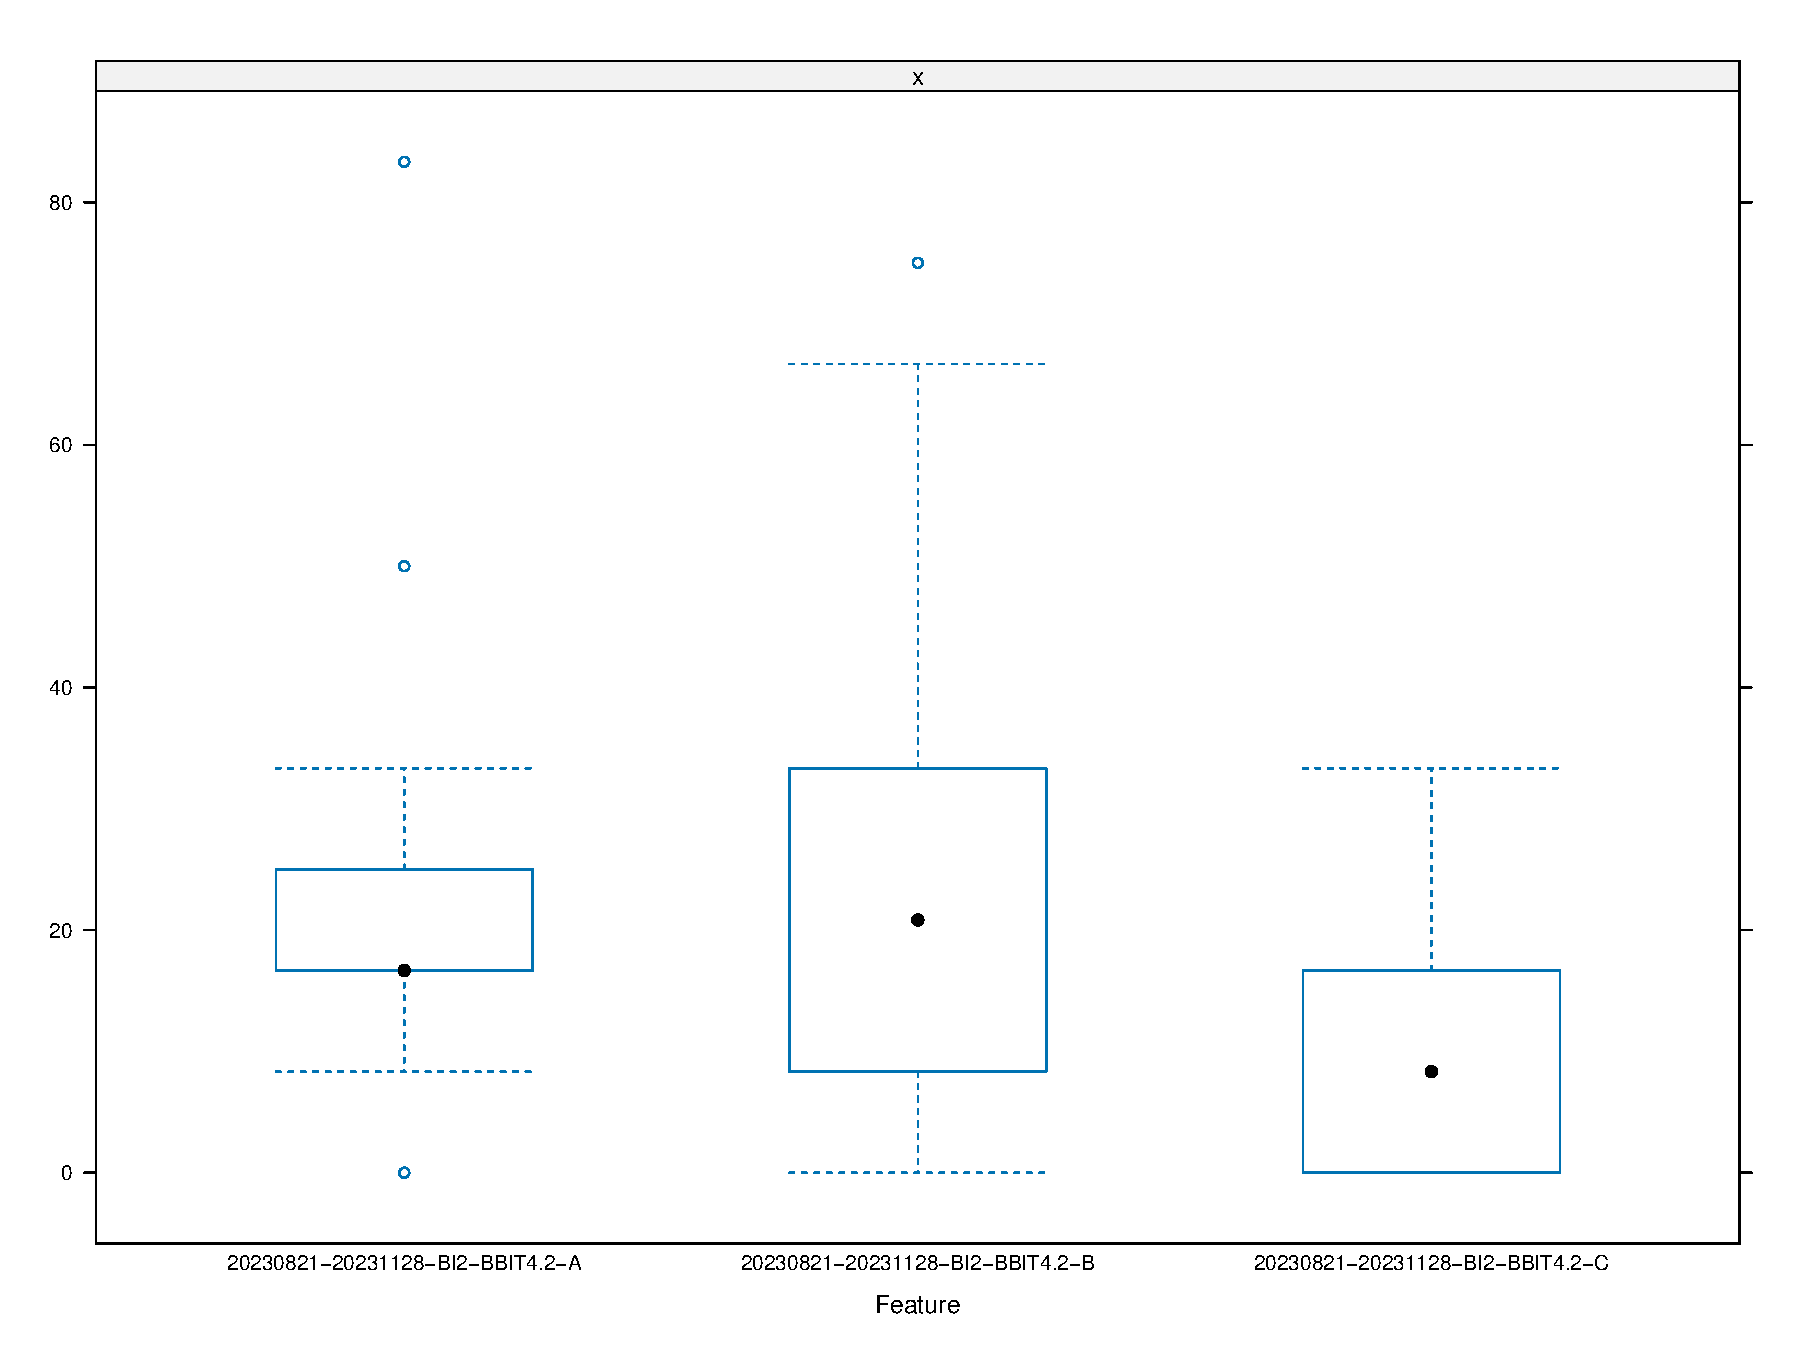
\includegraphics{AnalysisOfCourseEvaluation-Notebook_files/figure-latex/AbsenteeismBoxandWhiskerGroup-1.pdf}

\newpage

Absenteeism by specific class group:

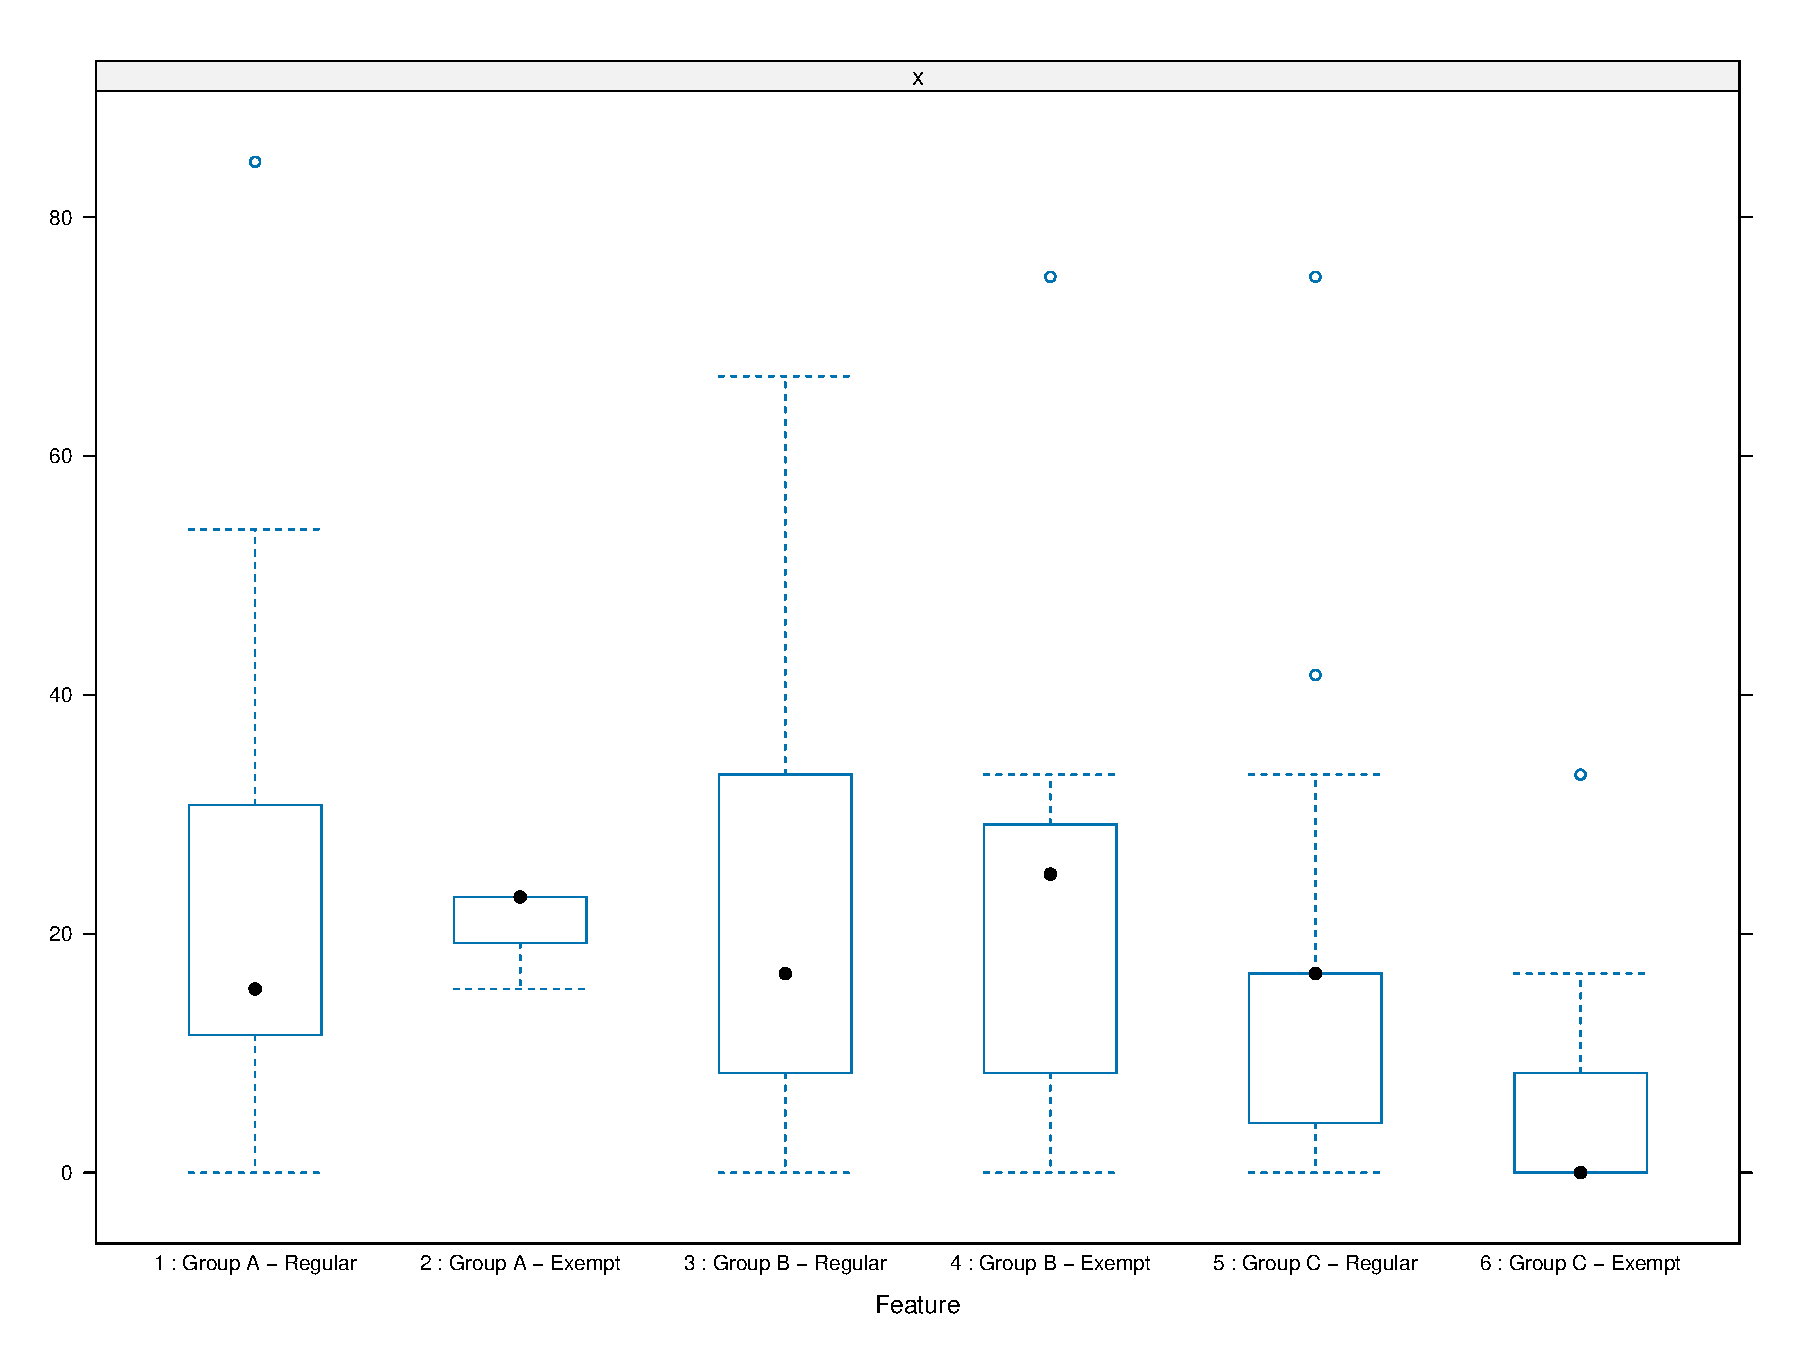
\includegraphics{AnalysisOfCourseEvaluation-Notebook_files/figure-latex/AbsenteeismBoxandWhiskerSpecificGroup-1.pdf}

\newpage

Absenteeism by gender:

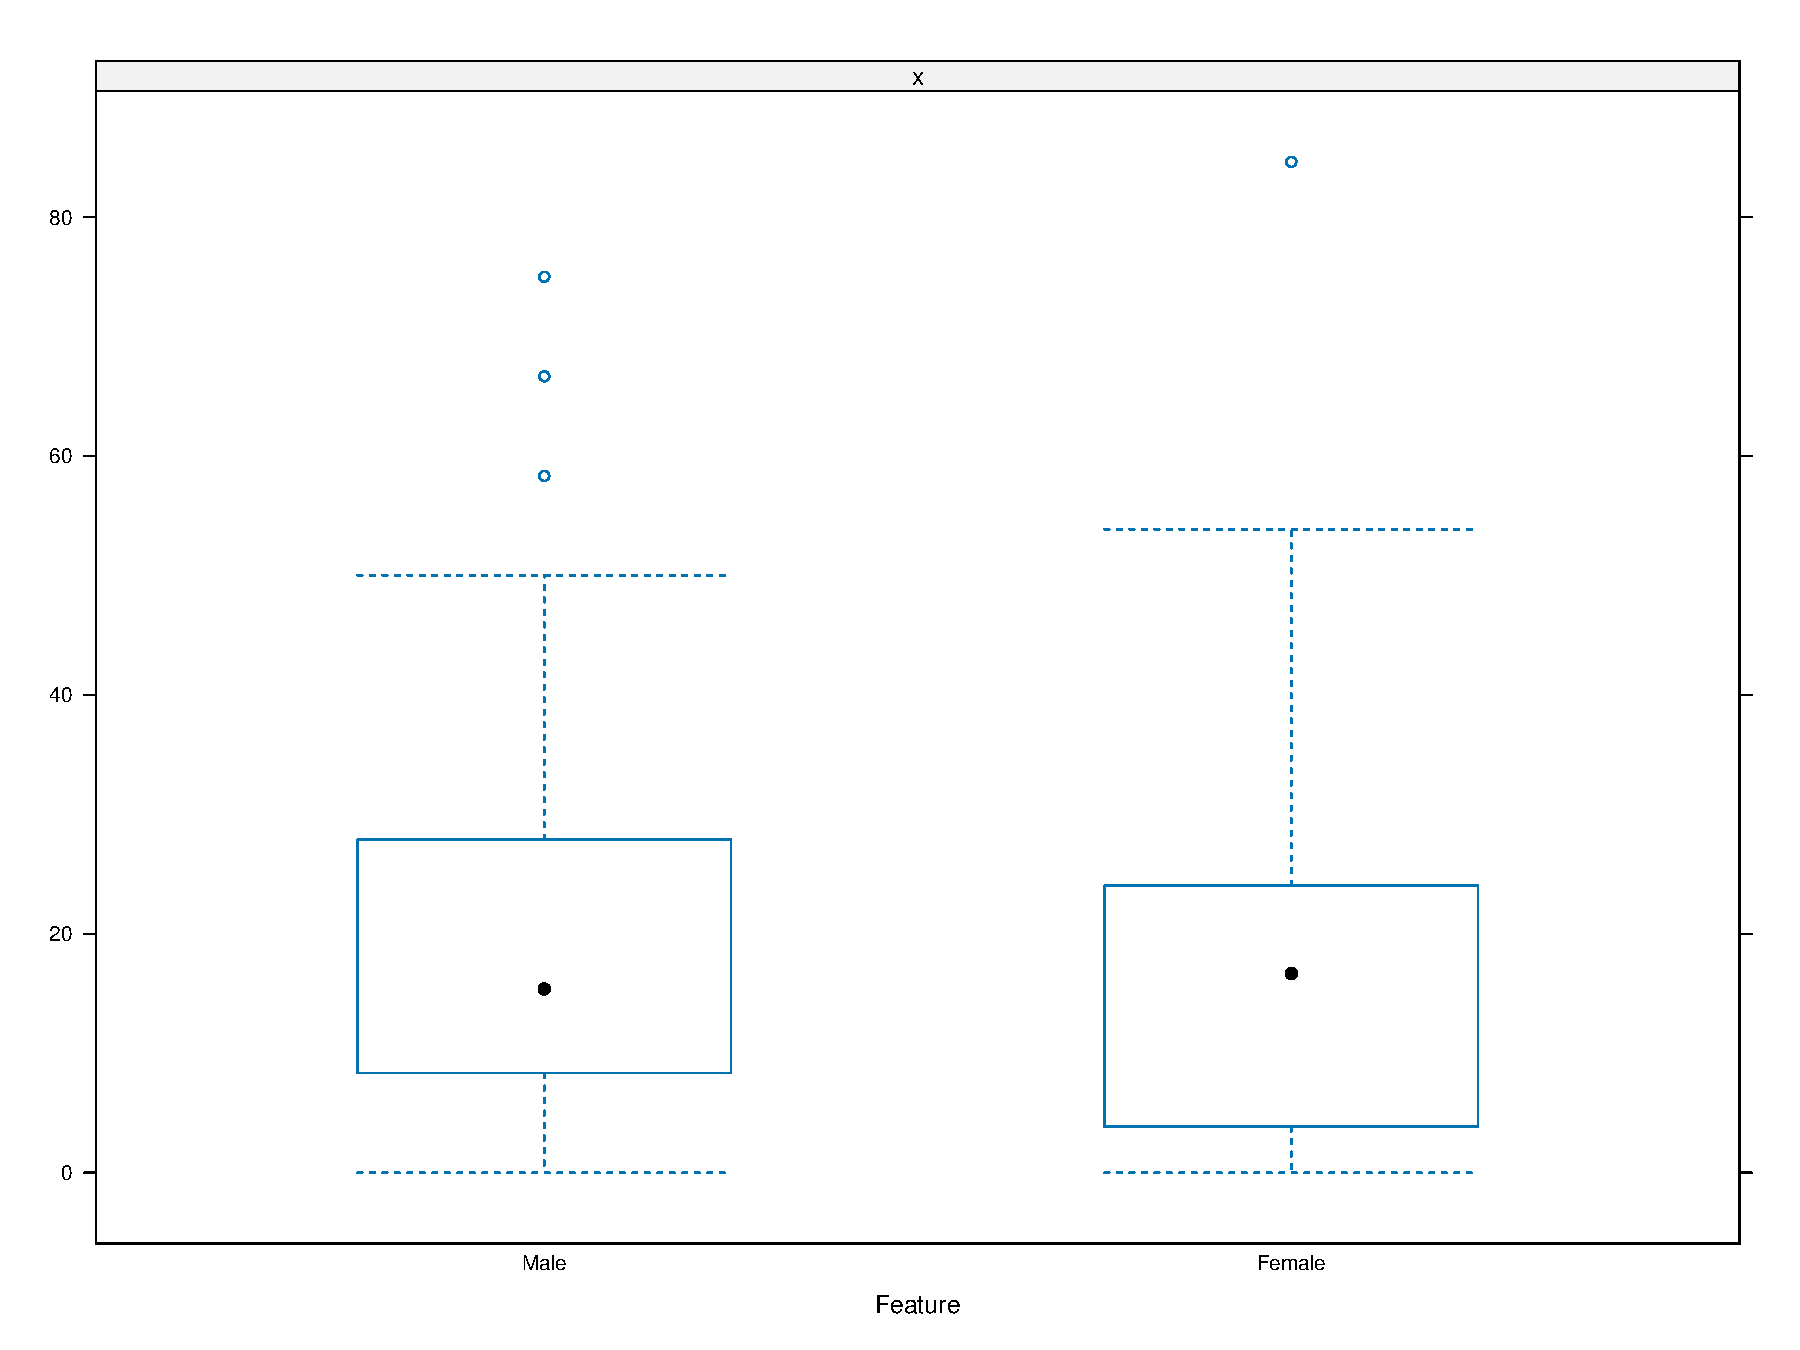
\includegraphics{AnalysisOfCourseEvaluation-Notebook_files/figure-latex/AbsenteeismBoxandWhiskerGender-1.pdf}

\newpage

\section{Qualitative Data (Likes and
Wishes)}\label{qualitative-data-likes-and-wishes}

\subsection{Term Frequency - Inverse Document Frequency (TF-IDF)
Score}\label{term-frequency---inverse-document-frequency-tf-idf-score}

The plot below presents the quantitative measure of ``significance''
using the Term Frequency - Inverse Document Frequency (TF-IDF) score:

TF-IDF Score (likes) per gender:

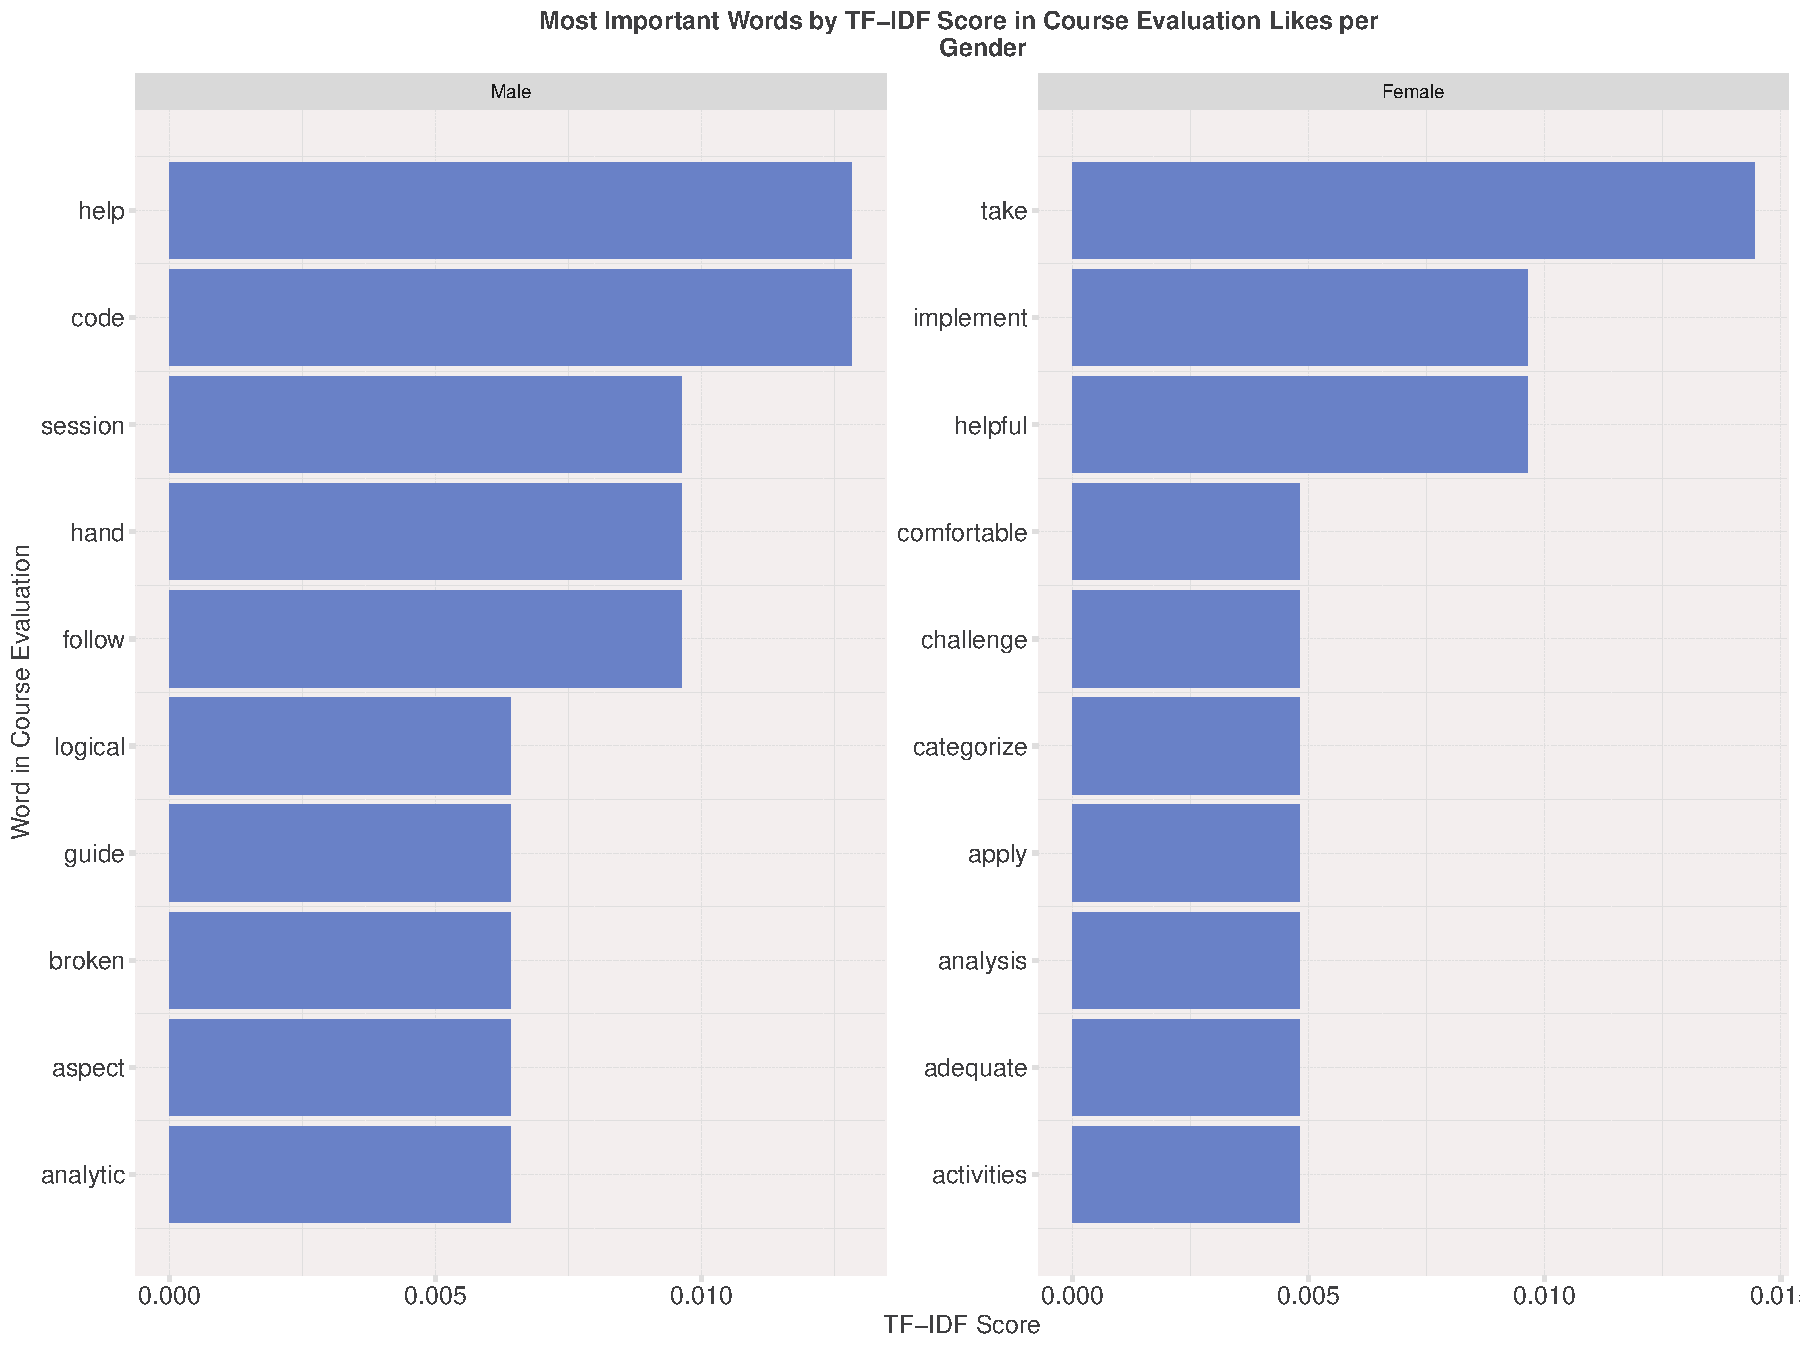
\includegraphics{AnalysisOfCourseEvaluation-Notebook_files/figure-latex/TF-IDFLikesPerGender-1.pdf}

\newpage

TF-IDF Score (likes) per specific class group:

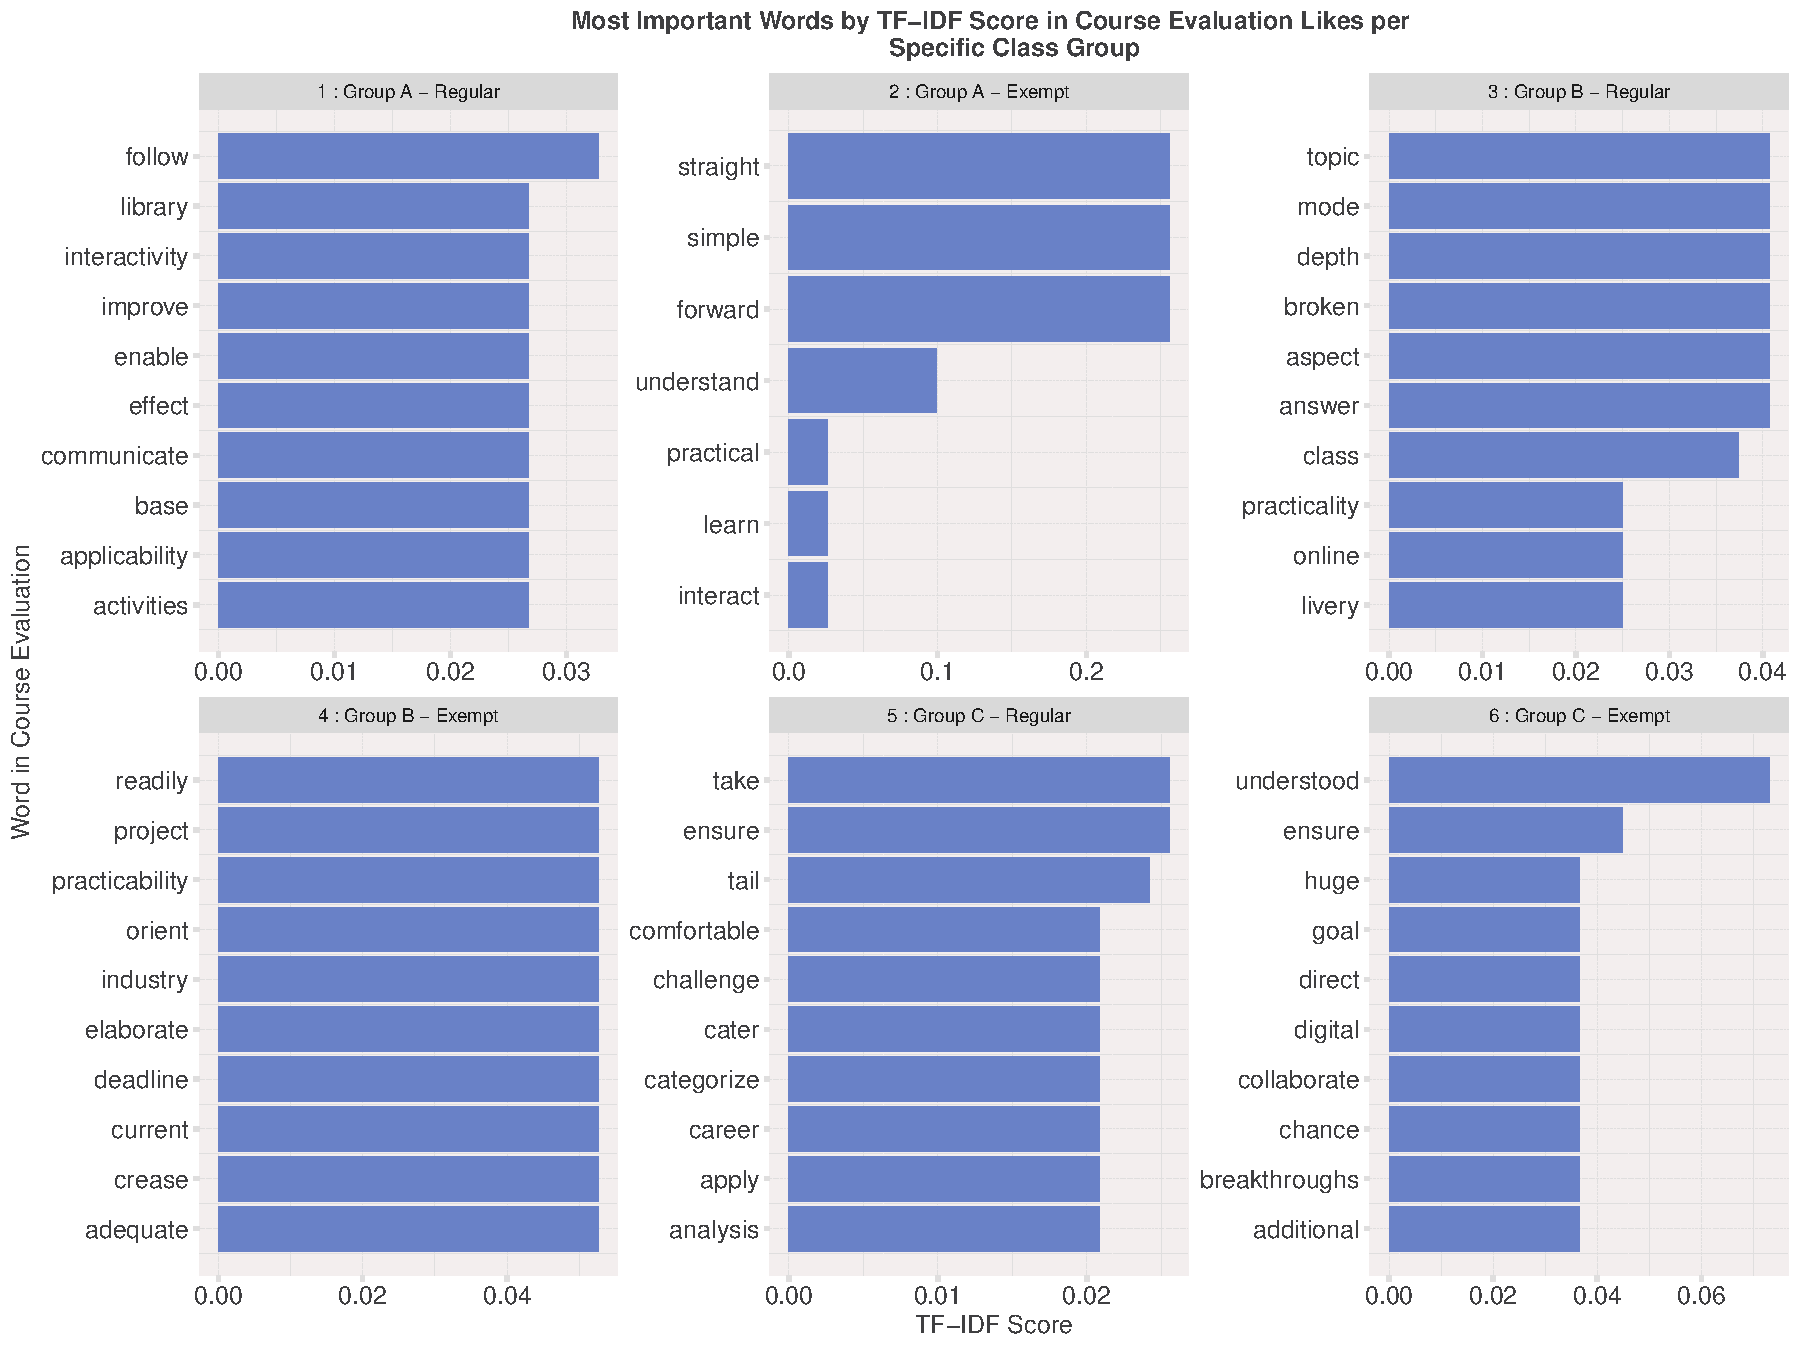
\includegraphics{AnalysisOfCourseEvaluation-Notebook_files/figure-latex/TF-IDFLikesPerGroup-1.pdf}

\newpage

TF-IDF Score (wishes) per gender:

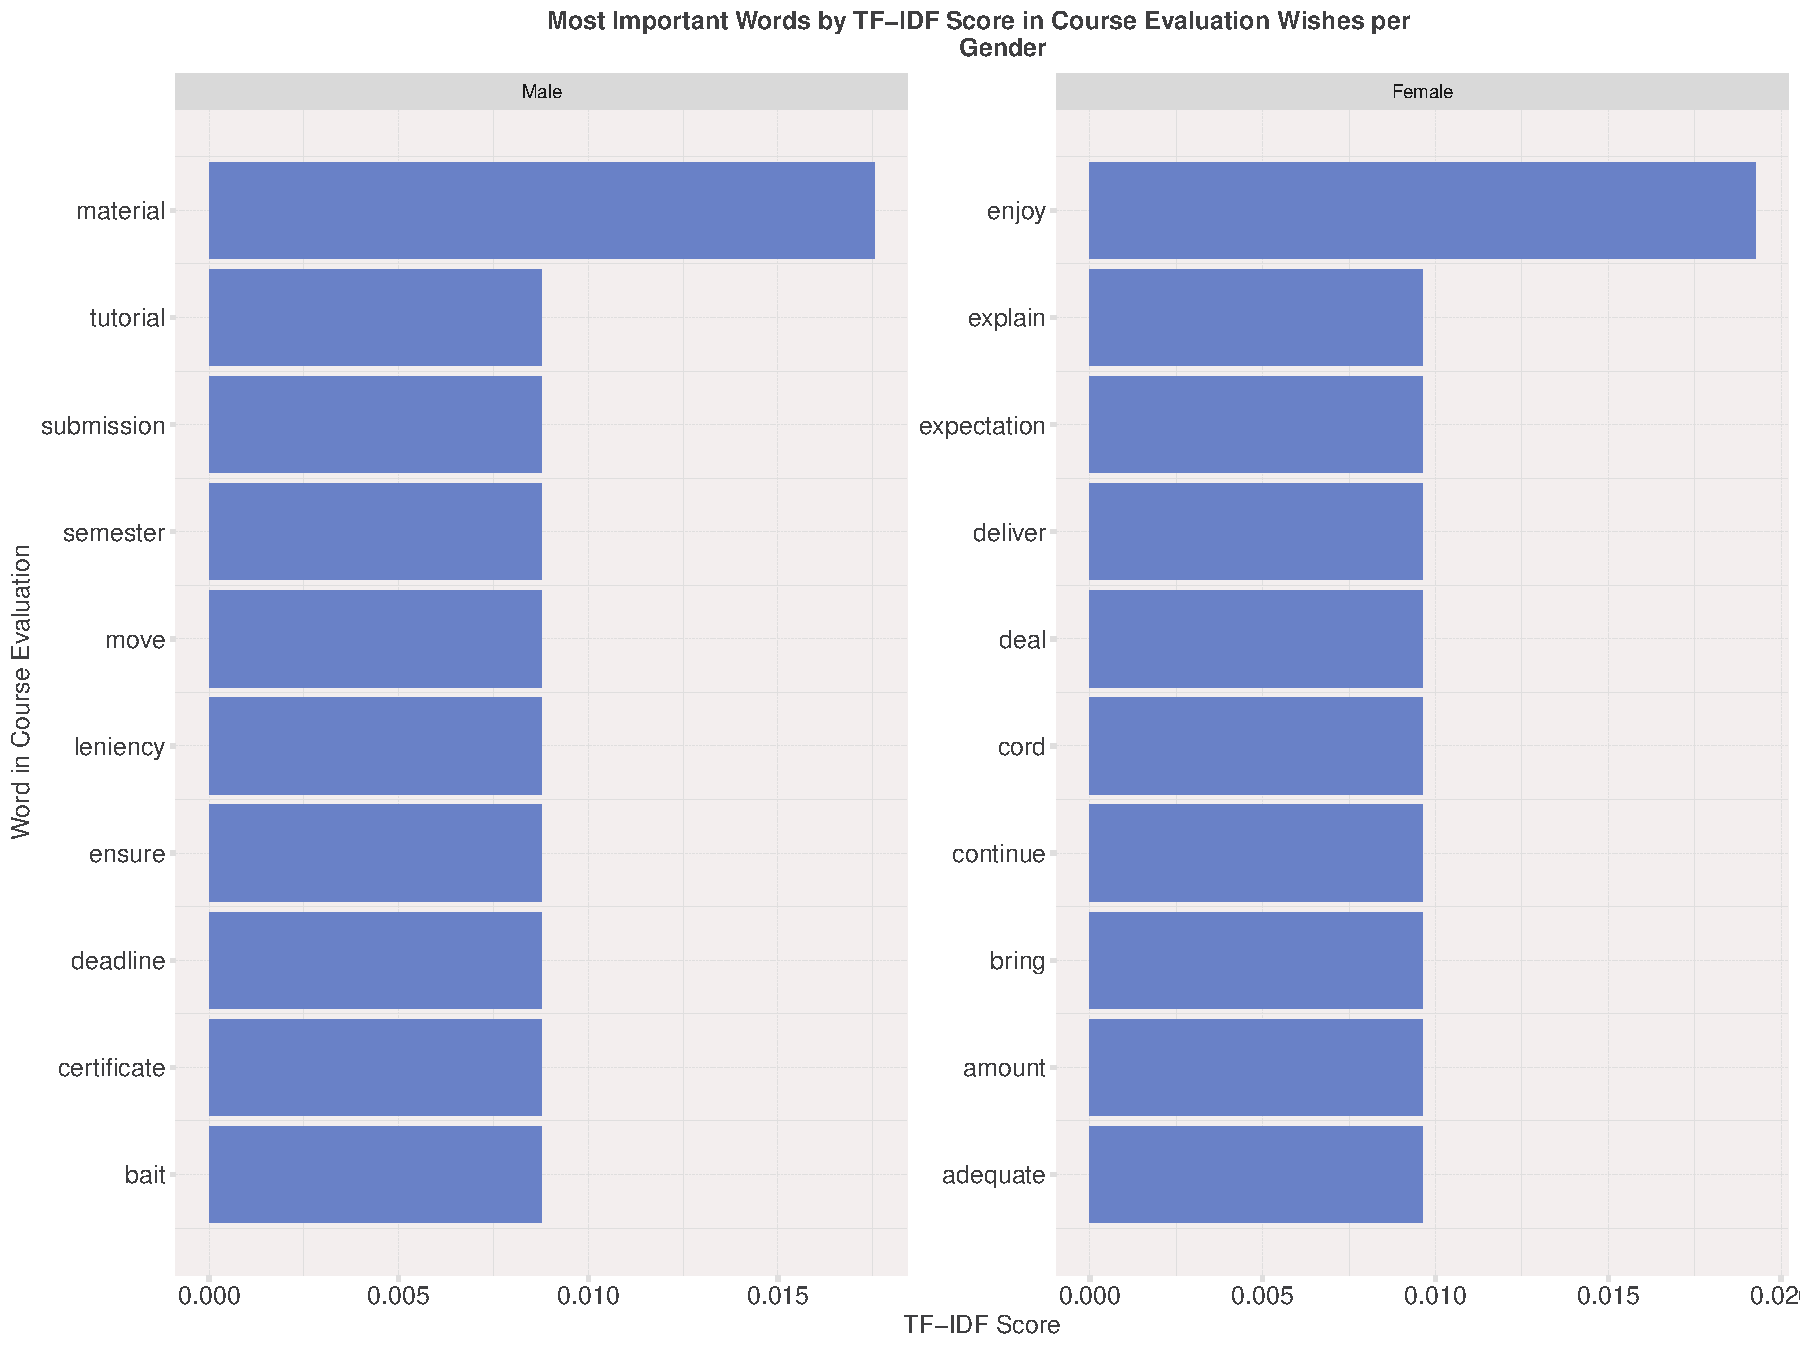
\includegraphics{AnalysisOfCourseEvaluation-Notebook_files/figure-latex/TF-IDFWishesPerGender-1.pdf}

\newpage

TF-IDF score (wishes) per specific class group:

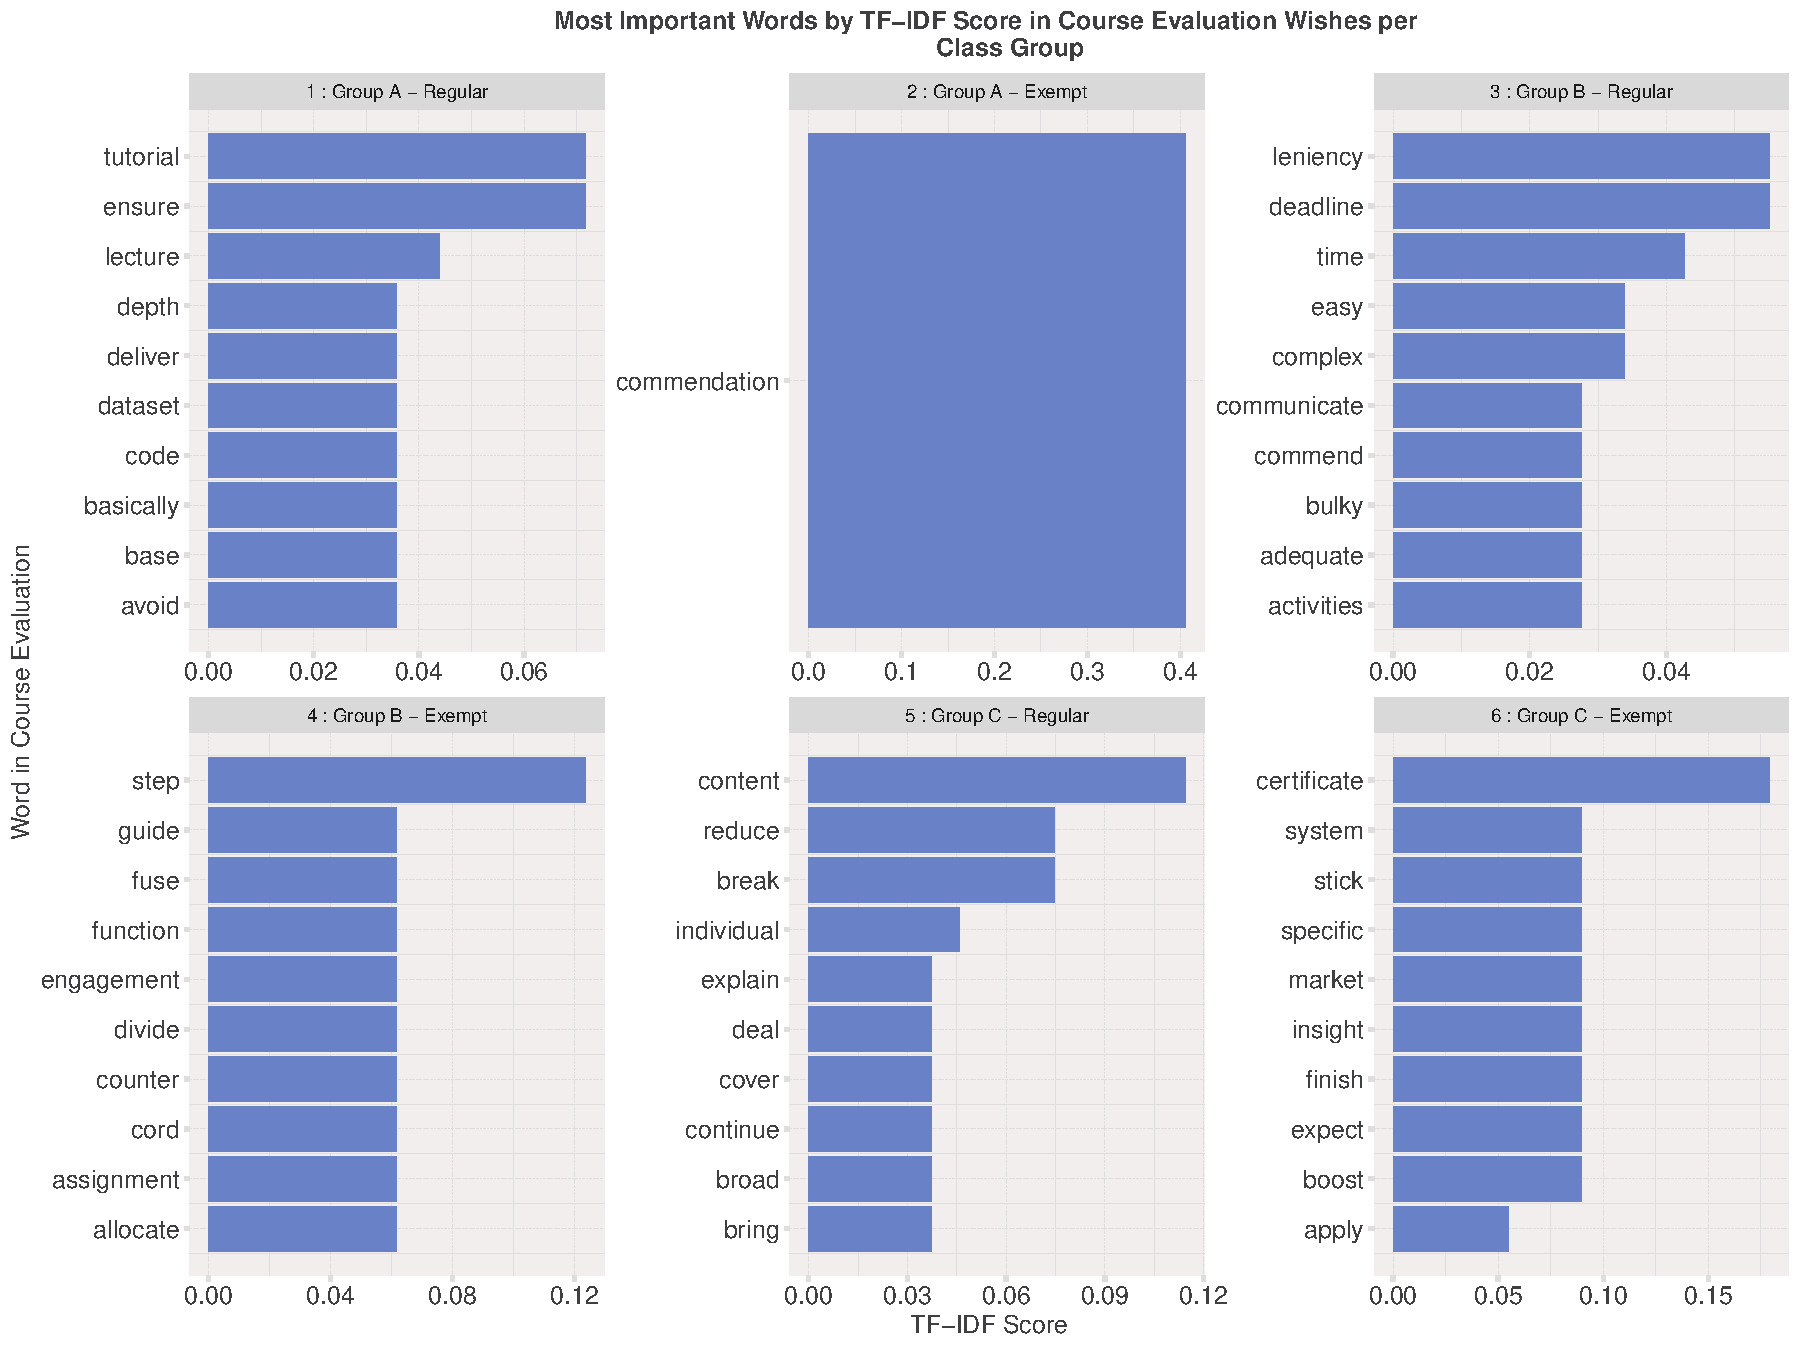
\includegraphics{AnalysisOfCourseEvaluation-Notebook_files/figure-latex/TF-IDFWishesPerGroup-1.pdf}

\newpage

\subsection{Lexicon-Based Sentiment
Analysis}\label{lexicon-based-sentiment-analysis}

The overall sentiment for the likes is:

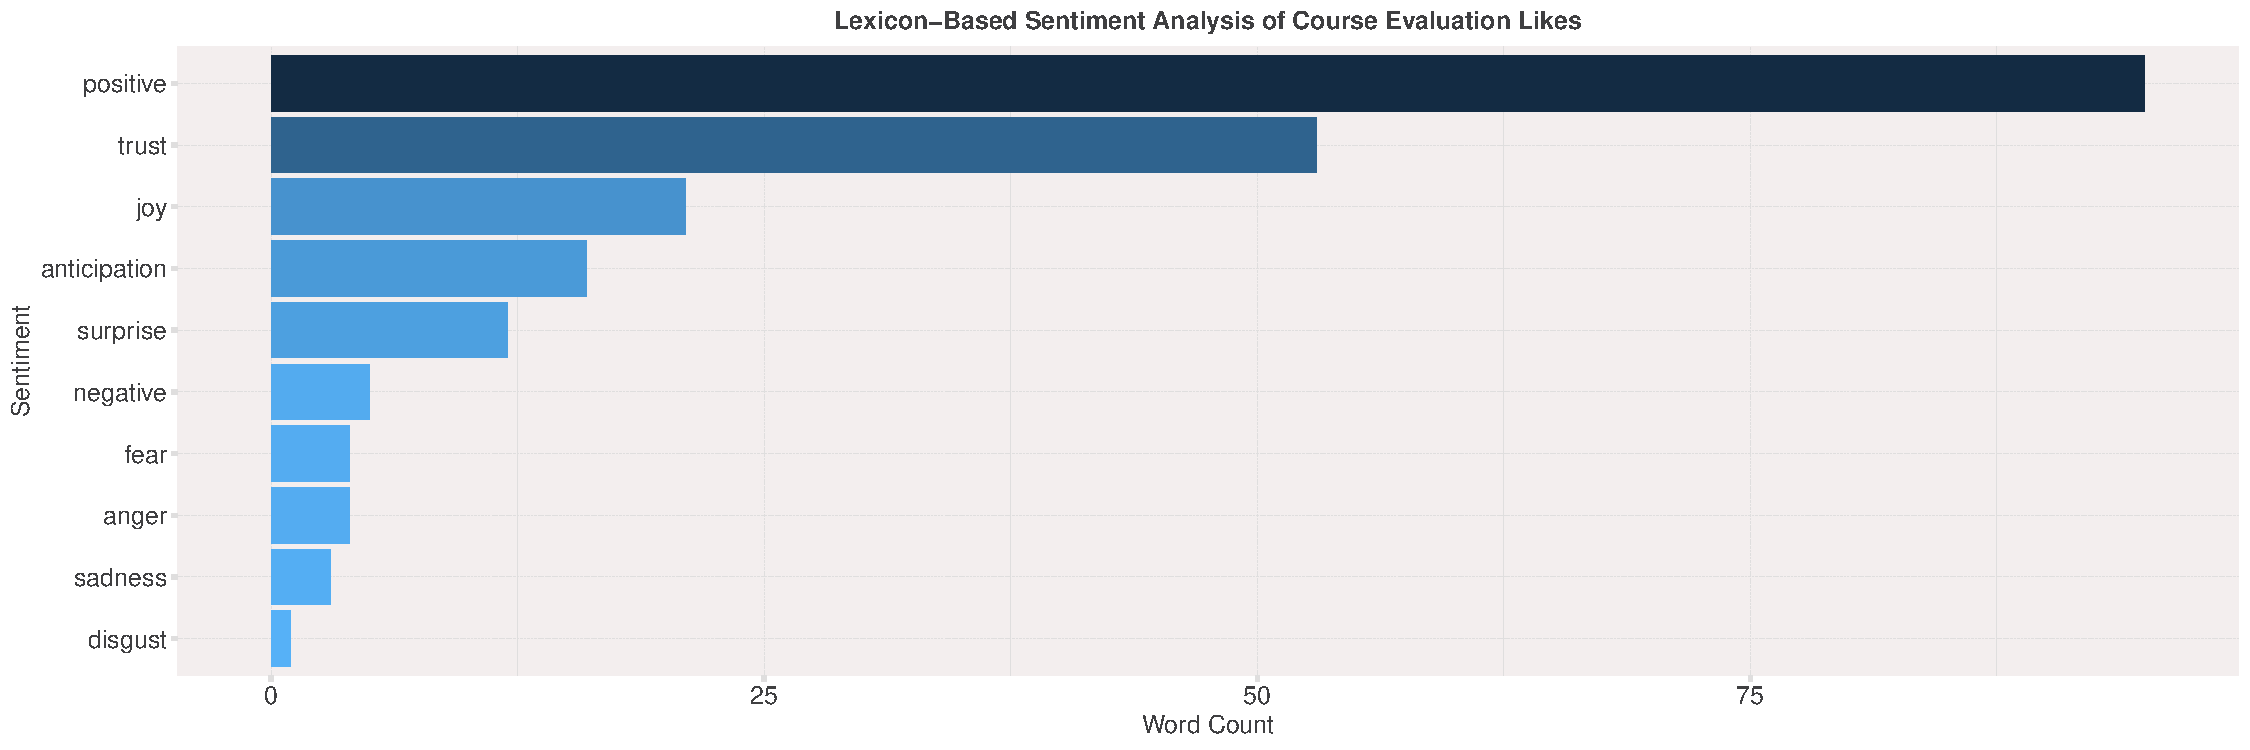
\includegraphics{AnalysisOfCourseEvaluation-Notebook_files/figure-latex/OverallSentimentForLikes-1.pdf}

\newpage

The overall sentiment for the wishes is:

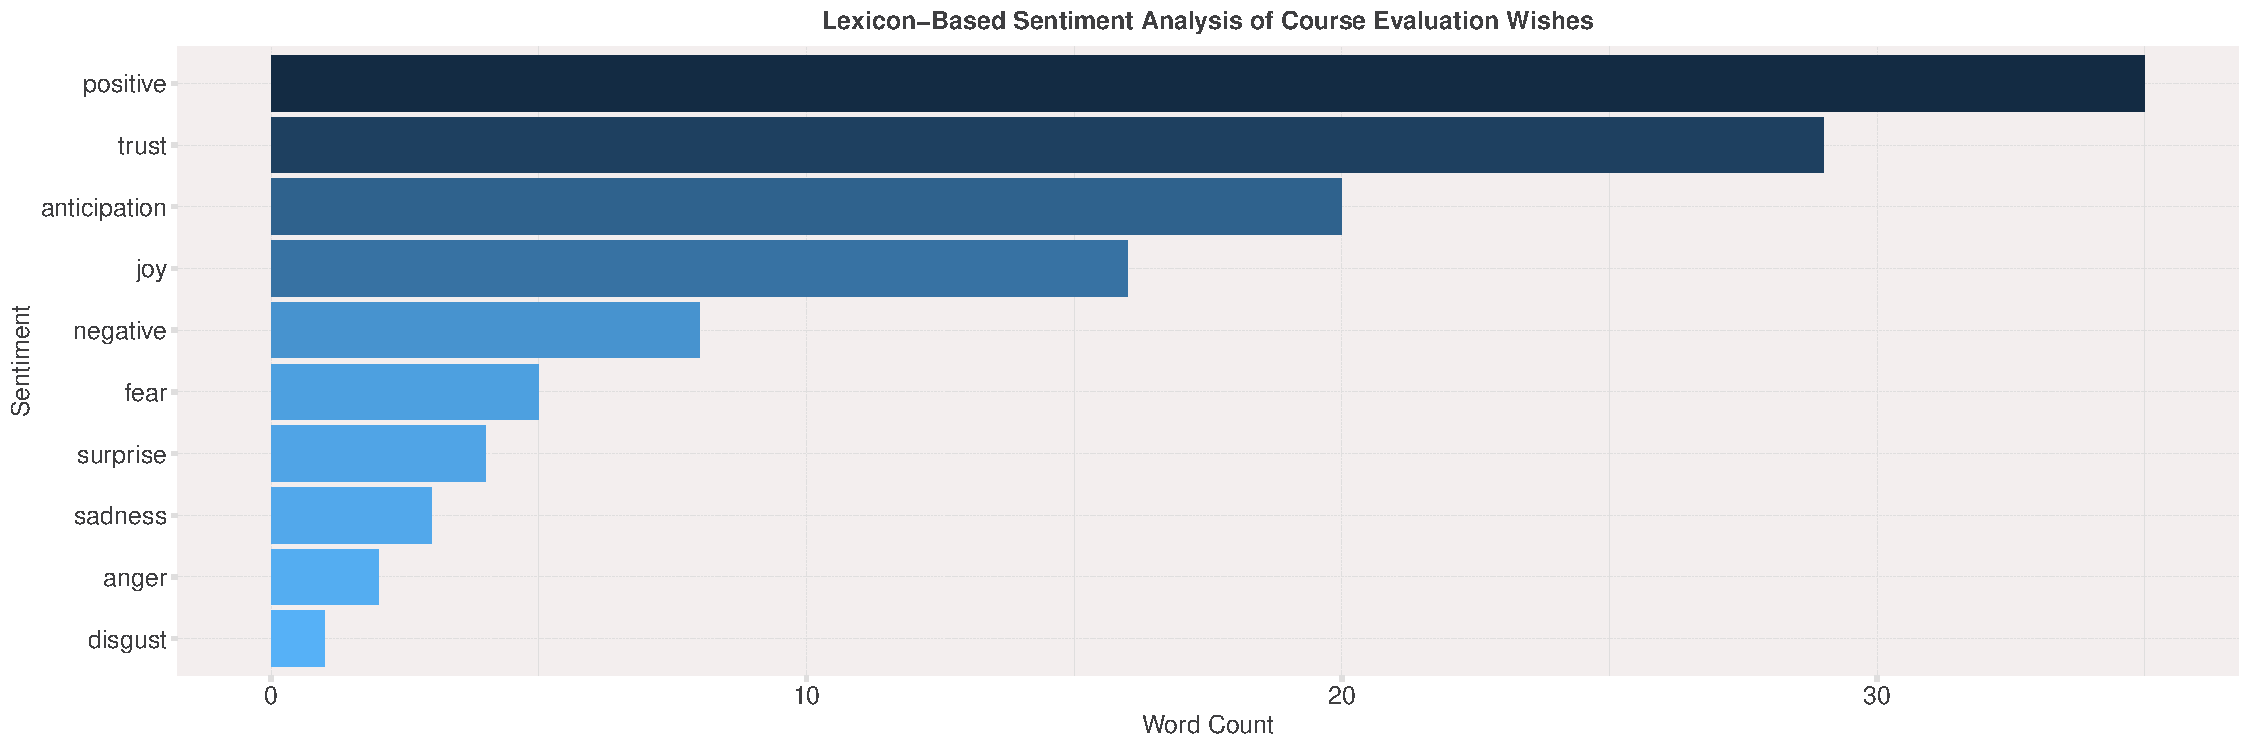
\includegraphics{AnalysisOfCourseEvaluation-Notebook_files/figure-latex/OverallSentimentForWishes-1.pdf}

\newpage

Chord Diagram of Likes per Class Group:

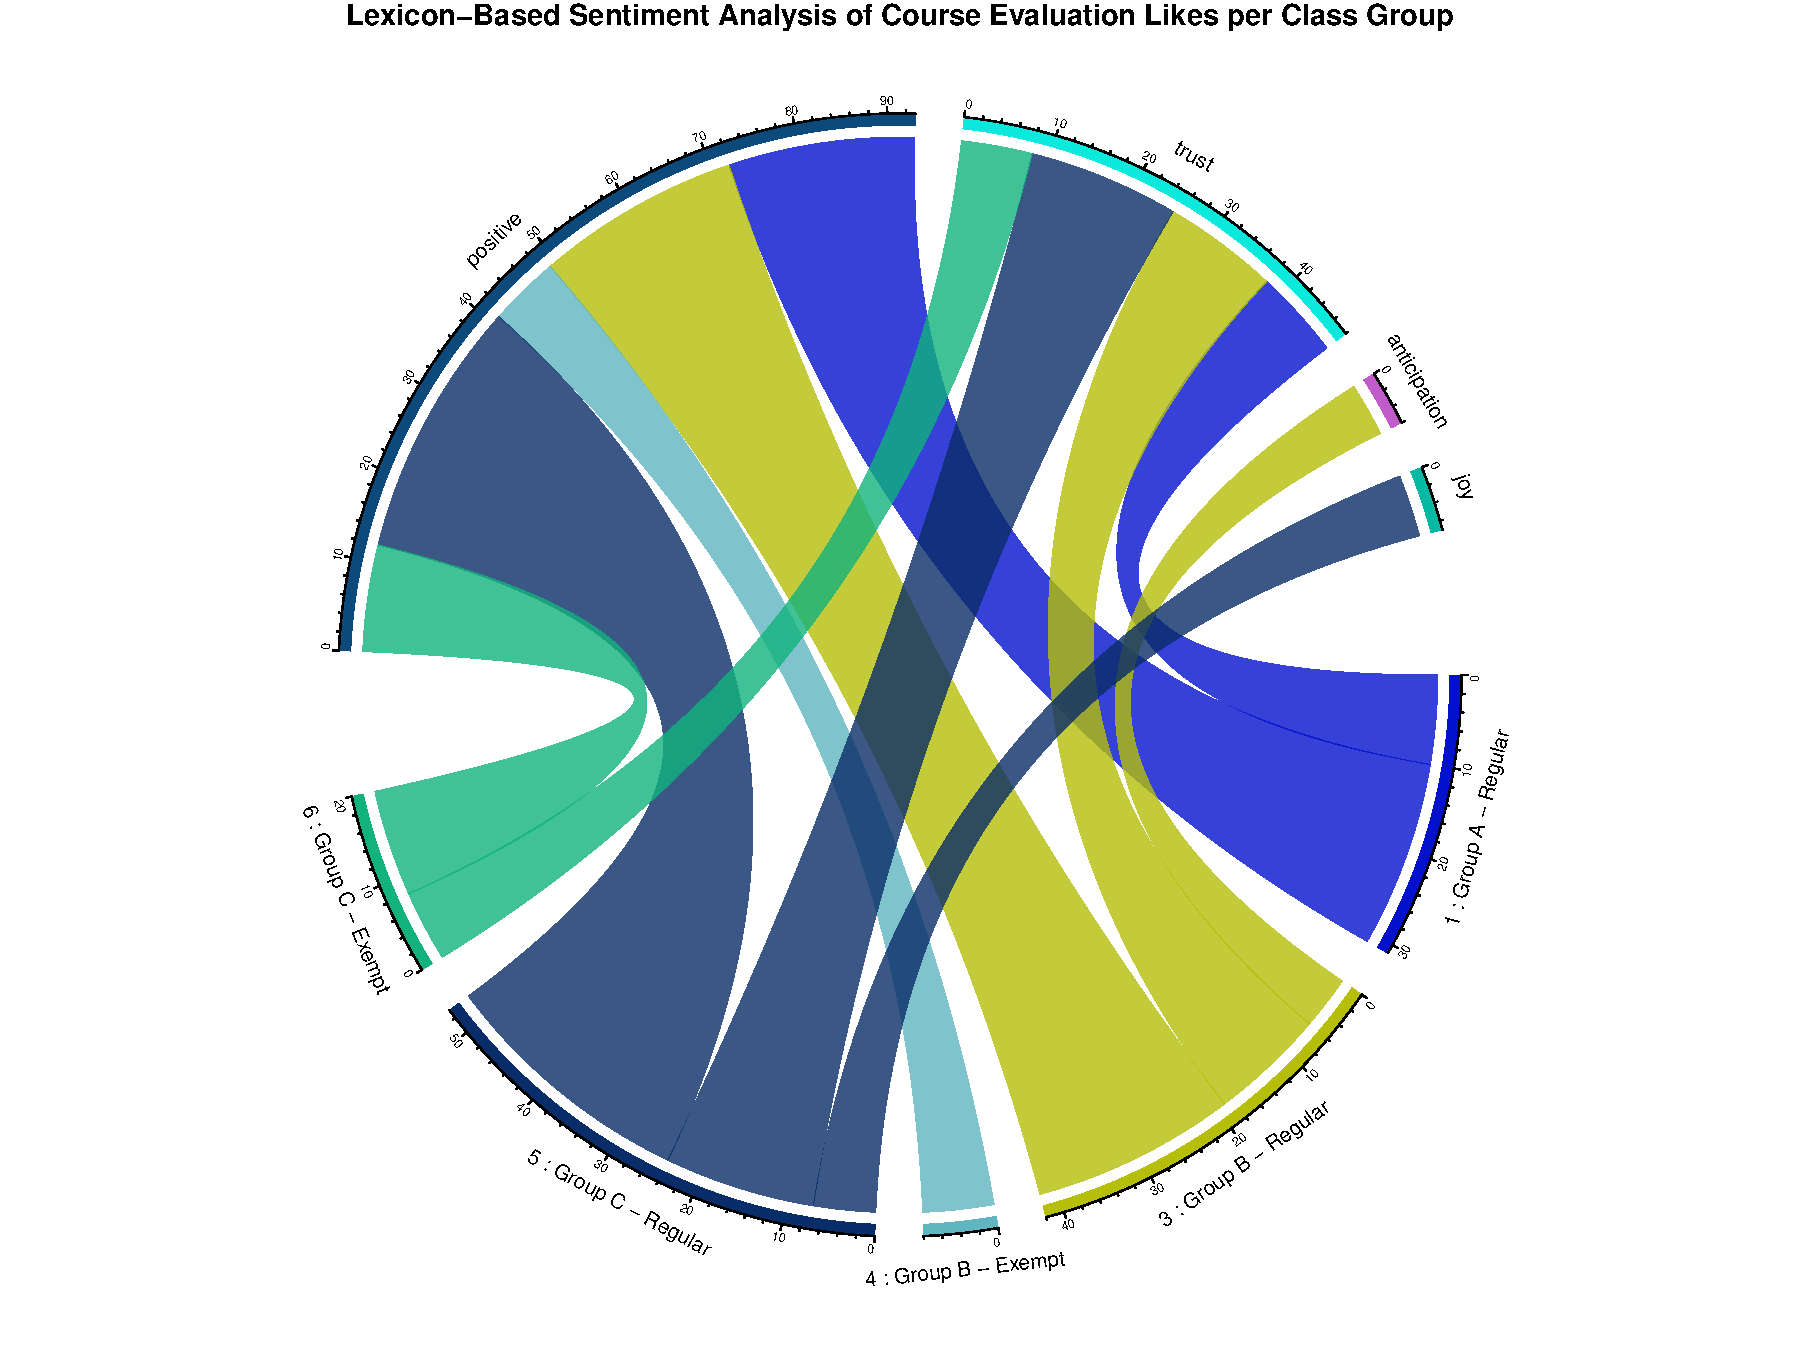
\includegraphics{AnalysisOfCourseEvaluation-Notebook_files/figure-latex/ChordDiagramLikesPerGroup-1.pdf}

\newpage

Chord Diagram of Likes per Class Gender:

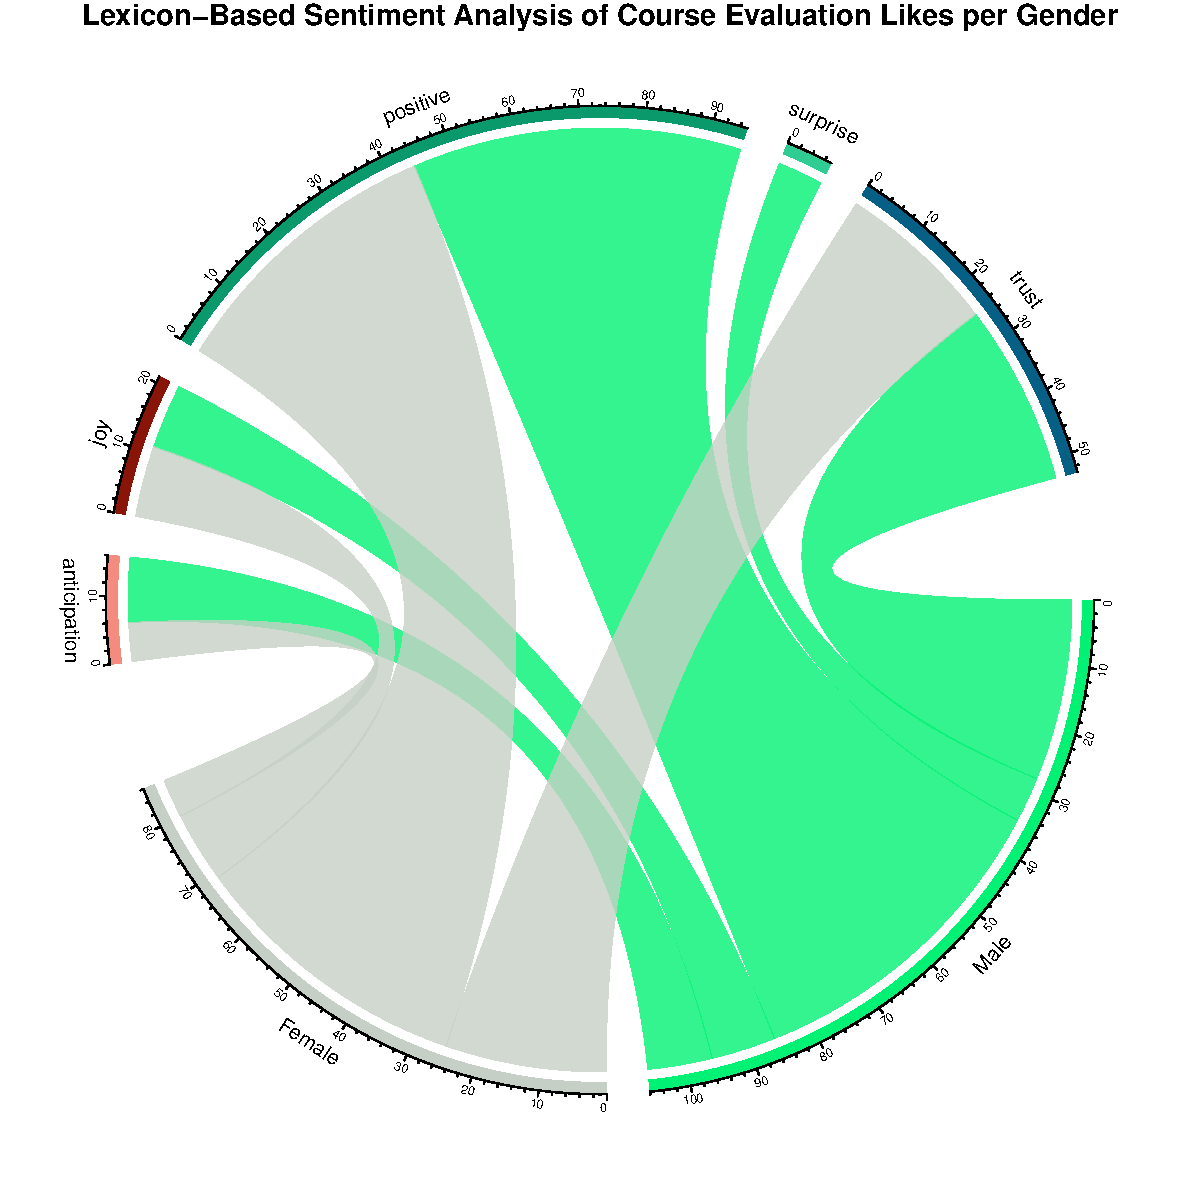
\includegraphics{AnalysisOfCourseEvaluation-Notebook_files/figure-latex/ChordDiagramLikesPerGender-1.pdf}

\newpage

Chord Diagram of Wishes per Class Group:

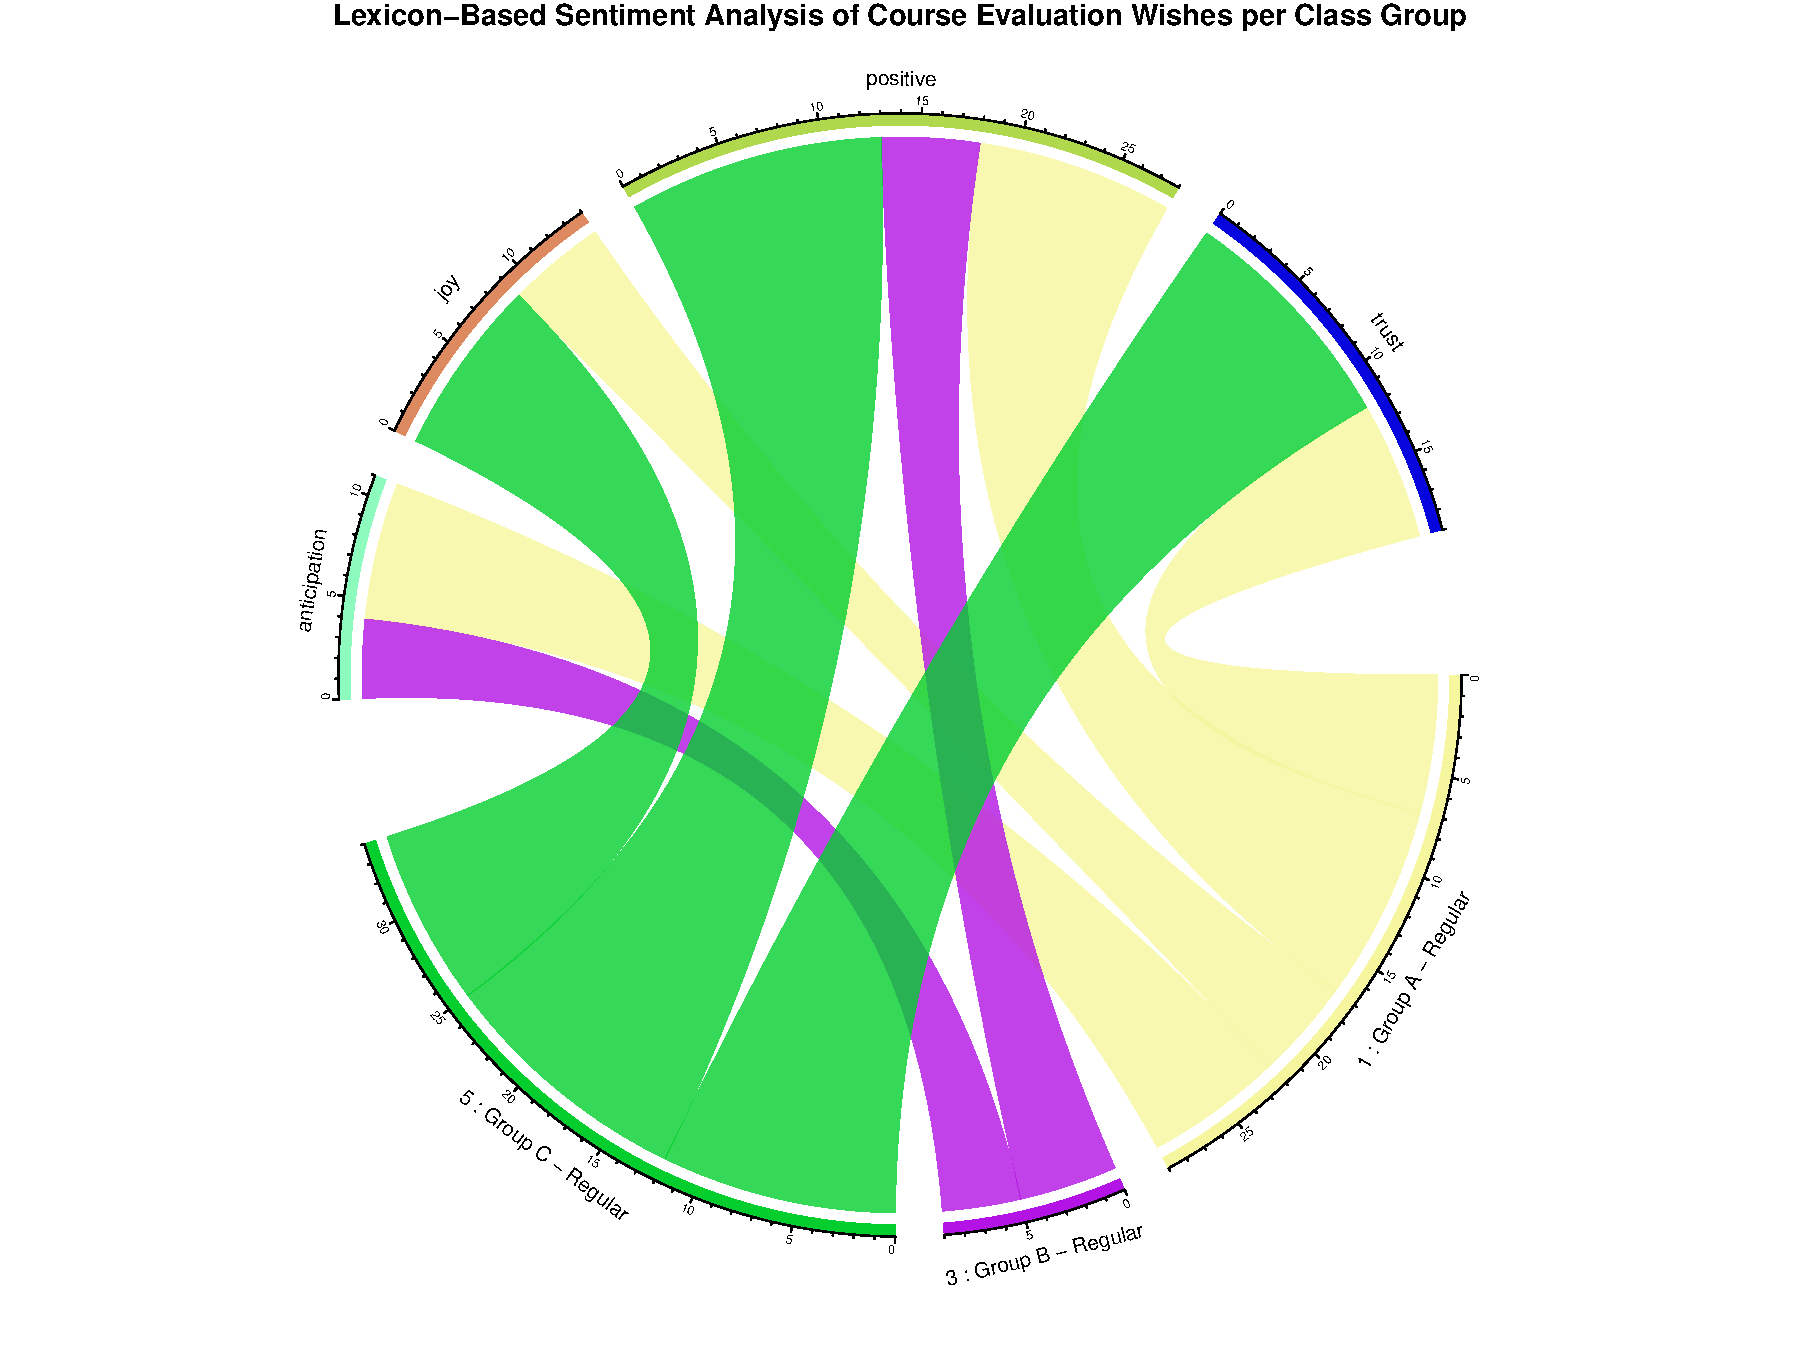
\includegraphics{AnalysisOfCourseEvaluation-Notebook_files/figure-latex/ChordDiagramPerGroup_Wishes-1.pdf}

\newpage

Chord Diagram of Wishes per Gender:

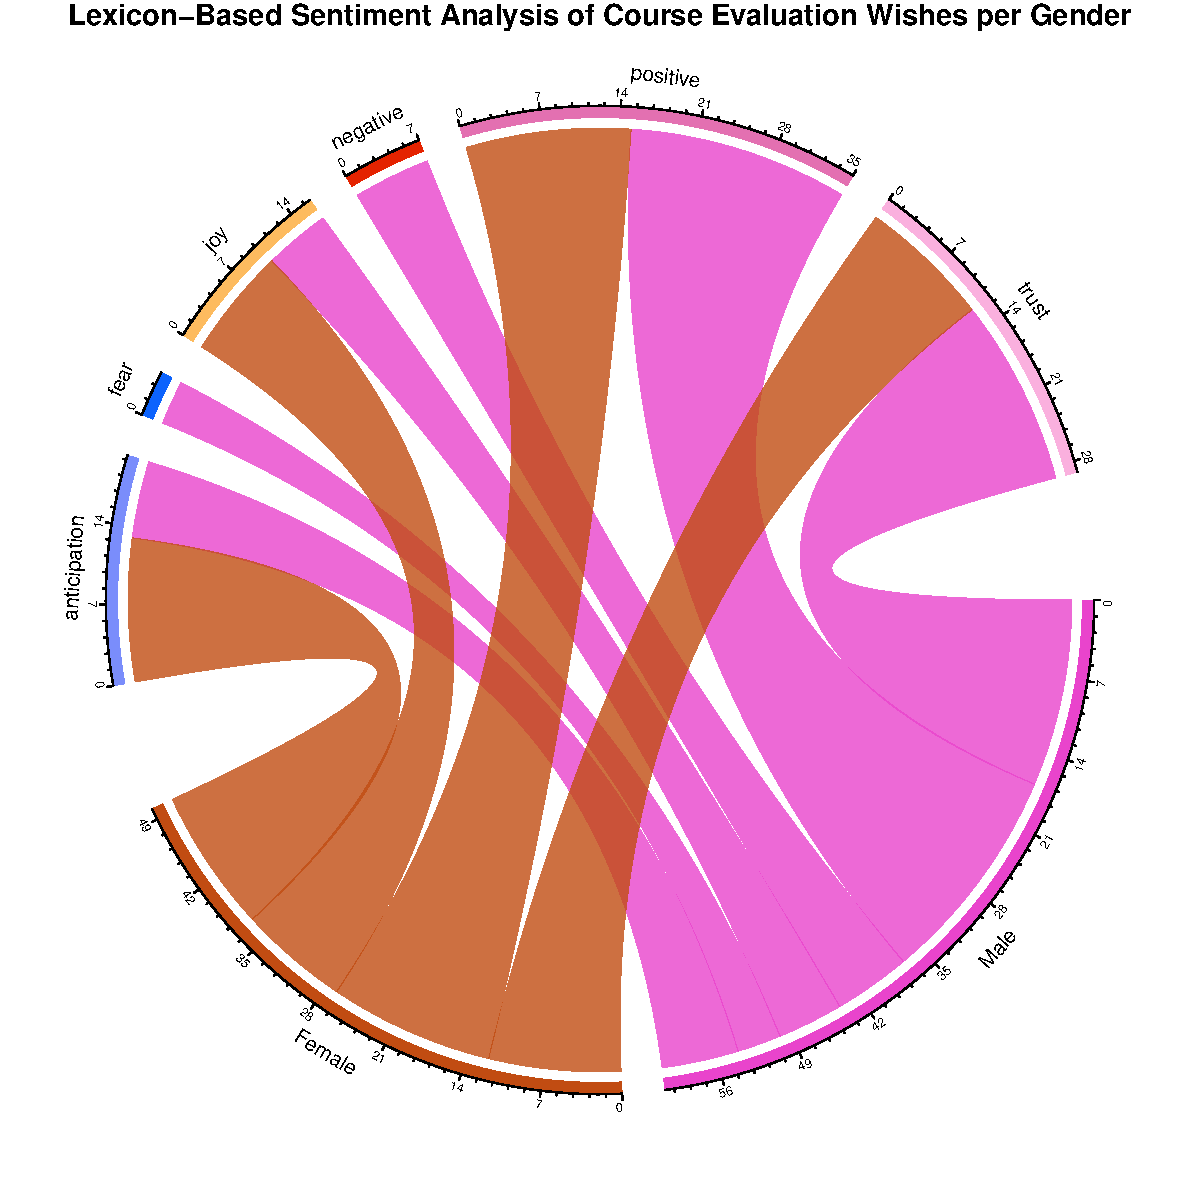
\includegraphics{AnalysisOfCourseEvaluation-Notebook_files/figure-latex/ChordDiagramPerGender_Wishes-1.pdf}

\newpage

\subsection{Raw Data}\label{raw-data}

\subsubsection{Likes}\label{likes}

The raw data of the likes is as follows:

Write two things you like about the teaching and learning in this unit
so far

x

It is interesting and helps improve coding skills

it is very detailed hence of great helpIt is interactive both in the
unit and in regards to other units such as IS project II

~Ensemble Methods for Predictive Analytics~ Predictive Modelling Using
R~

Interactive

The concepts are well explained Communication is effective~

It is a bit more practical due to the use of python and r The instructor
is well organized and the teaching methods are useful

It is practical and based on modern concepts The labs are interesting
and thought provoking

I like that the labs are practical I like being given enough time to do
the labs

Everything is good

It is interesting and interactive since we get to use different tools in
our sessions.

So far its been a hard unit and fortunately the teaching style for the
lecture is helping as he guides us along~

Lecturer is efficient classes start and end on time

Increase submission deadline~

The practical labs are engaging hence skill development~ the teaching
method and lectures~

\begin{enumerate}
\def\labelenumi{\arabic{enumi}.}
\tightlist
\item
  It is comprehensive 2. It is interesting.

  It is step by step ~

  \begin{itemize}
  \tightlist
  \item
    The content is really engaging and intense and shows that learning
    is there. - Also additional hands on skills like using GitHub and
    collaborations which plays a huge role in the personal development
    goals in the digital space.~

    N/A

    Interactivity and applicability of the unit

    The online classes The Labs that require submissions help me to dig
    deeper.

    The unit is very practical which helps me in the long run. The
    lecturer does not leave anyone behind, ensures everyone has
    understood the concept

    Work is clearly and easily broken down The lecturer is very
    available for consultation

    The teaching for this unit has been very comprehensive so far and
    engaging with the lecturer. The learning implements group works.

    Learning to use GIT Being taught practically and through
    walk-throughs

    The step by step explanation of the concepts is very helpful The
    time to complete the labs is sufficient~

    The lec takes his time to teach the concept

    Detailed Explanations. Quick feedback by lecturer.

    The lecturer is readily available to help when one is stuck The unit
    is well structured and organized

    Very in depth Very practical

    Its practical and has interactive learning~

    It is interactive~ It is engaging

    The lecturer does everything in his power to ensure we are
    comfortable with content being taught and make sure we are following
    along together.~The e-learning site is also very well organized and
    categorized for this unit

    Answers the questions asked Explains well

    Patience and flow

    mode of delivery Information

    The mode of delivery~ The assistance of reference links put on
    elearning for easy reference~

    The lecturer ensures everyone understandsThe labs are fun

    The lecturer ensures everyone has understood. It is practical.

    The explanations to the various concepts are well explained~

    the labs sessions are nice

    i like the group labs i like the topics

    I find it current industry oriented

    The lecturer provides adequate feedback on the questions asked. The
    lab work clearly elaborates on the work taught.

    The lecturer explains the content really well.

    Takes time to organize his work, I appreciate the effort

    So far so good The lecturer is very clear

    It is comprehensive It is easy to follow

    Labs that describe each step to be followed are engaging and
    learning enables me to follow through the lab properly It is very
    engaging and interactive.

    The lecturer asks questions The lectures are clear~

    Interactive Interesting~

    The assistance by the lecturer, the practicality

    Lab work Class sessions

    ~It is very participative and lecturer gives room for questions

    feedback is quickLecturer is willing to help

    Working as a team

    the fact that we get to do the lab work in groups~ the interactive
    online and on campus classes

    I like how the Lecturer explains the concepts and takes us through
    the labs

    The concept are explained very well A chance to learn R I have
    wanting to interact with R and data

    very interactive and hands on

    on hand Practice Good delivery

    It's interactive and very logical.

    The technical aspect of the unit. The attentiveness to detail when
    it comes to the labs and concepts are clearly explained.

    Wide scope of content Practicability

    Once you follow the steps for the lab you will be okay. The lecturer
    helps in one on one for the labs if one has an issue

    I like the way the topics are broken down very logical and easy to
    understand. I like that we are constantly able to ask questions and
    be answered regardless of the nature of the question.

    The lectures

    Its Good

    the lecturer the lectures

    Lecturer, Teaching method

    I like this ui=nit because it prompts me to think actually think and
    connect the dots~

    Well explained content

    Gaining R skills

    Use of realistic~ code group work

    practicality Engagement

    Group Labs

    its straight forward and simple to understand~

    I like the practicality of R and learning github in depth through
    the group work

    Group workPractical Exercises

    The learning of this unit is good in terms of the detailed and step
    by step practicals shown by the lecturer for each lab.The
    recordings.

    I like that it challenges me to apply everything practically.

    None

    The practical aspect. The group work is good.

    Labs activities, Quizzes help a lot on learning during the semester

    clear and direct to the point~ step by step teaching works for me

    The lecturer explains everything in detail and caters for both ides
    that is vscode and rstudio

    N/A

    N/A~

    How to use and implement R as a language for data analysis

    I am learning to use new language, R language, and how to use it
    together with the available libraries for predictive analytics. ~

    Its practical~

    It is very practical and a good example of a prospective career path
    for many.

    \begin{enumerate}
    \def\labelenumii{\arabic{enumii}.}
    \tightlist
    \item
      The lecturer makes the content easy to understand

      the teaching method the recording being online is also helpful~

      The practicals
    \end{enumerate}
  \end{itemize}
\end{enumerate}

\newpage

\subsubsection{Wishes}\label{wishes}

The raw data of the wishes is as follows:

Write at least one recommendation to improve the teaching and learning
in this unit (for the remaining weeks in the semester)

x

none

i would like if the concepts were divided where we learn the functions
first online then do the practicals of it in person

N/A

Flexibility

I don't have any~

Leniency with regards to lab work submission and future project work

More tutorials based on the labs

Use of less complex datasets

i have no recommendations

A guide to help us counter different problems like installation of
packages during labs.

I would like lab exercises to be done more in class so as to easily
understand~

Lecturer might be a bit fast at times

Step by step materials/videos on how to do the lab works~

student involvement~~

\begin{enumerate}
\def\labelenumi{\arabic{enumi}.}
\tightlist
\item
  Nothing

  Go easy on us abit, it is te last semester

  \begin{itemize}
  \tightlist
  \item
    To give us insights or recommendations about certifications that we
    can as well do, related to this unit which will boost our C.Vs for
    the interested students.~

    N/A

    A bit more tutorials on technical errors such as ones on knitting
    and rendering the markdown files

    If the concept requires many practicals, the classes should be more
    online.

    For the physical class to be moved to a lab

    Being more lenient with lab work

    Everything is okay so far.

    Sticking to a specific~application to be used

    No recommendation at the moment

    None

    The content is too broad and covers a lot i.e new softwares which
    make the unit overwhelming.

    It would be better if the physical classes were being recorded
    because at times one might be behind or missed an important lab step
    ~

    No recommendations

    N/A

    Make the course work less bulky and complex

    no comment

    n/a

    Too much content to deal with

    time liniency

    That the labs should be given more time to them~

    Breaks in between classes

    Nothing. I am enjoying and understanding the course.

    None~

    increase more labs

    the labs are quite hefty so it really makes the work easier to do in
    a group

    More engagement

    More time to be allocated in the lab work assignments.

    Nothing

    I am content

    Reduce content Reduce labwork

    .

    Proper detailed explanation of the labs, rather than rushing through
    them quickly~ More time is needed for lab completion and progressive
    follow-up so the lecturer knows where you are stuck.

    More time for labs

    So far none

    Reduce the workload, its honestly too much

    More reference material Breaks during classes at least 5 mins ~

    None\ldots.The unit met my expectation and was delivered perfectly

    Avoid online classes

    Deadlines to be extended abit

    N/A

    i am enjoying the unit as it is

    Since we are about to finish our 8.4.4 system. To give us more
    recommendation on certificates and what the job market expects from
    us

    better communication of activities btwn the students and the lec~

    .

    Ensure that the code work can work with any dataset and not fixated
    on provided dataset

    I would like there be more simpler labs with easier datasets to
    understands the concepts first then move on to more complex data
    handling and manipulation.

    None so far

    Kindly share more reading materials and past papers.

    I recommend that the deadlines on the labs be more flexible as there
    are many subject and projects running concurrently.

    The labs are long, they are individually basically the same size as
    an entire same project

    No recomendation

    so far so good

    Greater in depth exploration into labs to ensure we're actually
    understanding what is going on.

    The content is so hard to understand and the lec solving other
    people's issues only bring more confusion to some of us, I wish he
    would go through the content first then afterwards focus on
    individual problems

    He is doing a good job

    Personally I use linux and its kinda hard for me~ You can add some
    YouTube materials~

    Lab submissions still very confusing

    More online sessions

    None

    so far so good

    Adequate time for completing the labs

    More group work, less individual work

    ~No recommendations there is good delivery.

    One recommendation may be to explain how these concepts can relate
    to and apply to our IS Project 2.

    None

    It is okay.

    \begin{itemize}
    \tightlist
    \item
      Slide are very long (too much content) lecture can improve on
      that-

      nothing really

      There are many labs

      N/A

      N/A

      No comment, everything is fine

      None

      nothing all is well

      n/a.

      N/A

      so far I have been struggling a little with the Lab a bit but i'm
      hoping it will get better as we continue with the other labs

      N/A
    \end{itemize}
  \end{itemize}
\end{enumerate}

\end{document}
